%% LyX 2.0.0 created this file.  For more info, see http://www.lyx.org/.
%% Do not edit unless you really know what you are doing.
\documentclass[oneside,english]{amsart}
\usepackage[T1]{fontenc}
\usepackage[latin9]{inputenc}
\usepackage{geometry}
\geometry{verbose,lmargin=1in,rmargin=1in}
\usepackage{float}
\usepackage{booktabs}
\usepackage{amsthm}
\usepackage{amssymb}
\usepackage{mathdots}
\usepackage{graphicx}
\usepackage{esint}
\usepackage{tikz,pgfplots}
\pgfplotsset{compat=1.3}
\usetikzlibrary{plotmarks,shapes,arrows,positioning}

\DefineNamedColor{named}{mitred}    {rgb}{0.6,0.2,0.2}
\DefineNamedColor{named}{mitgray}   {rgb}{0.4,0.4,0.4}
\DefineNamedColor{named}{darkgray}   {cmyk}{0,0,0,0.90}


\makeatletter

%%%%%%%%%%%%%%%%%%%%%%%%%%%%%% LyX specific LaTeX commands.
%% Because html converters don't know tabularnewline
\providecommand{\tabularnewline}{\\}
\floatstyle{ruled}
\newfloat{algorithm}{tbp}{loa}
\providecommand{\algorithmname}{Algorithm}
\floatname{algorithm}{\protect\algorithmname}

%%%%%%%%%%%%%%%%%%%%%%%%%%%%%% Textclass specific LaTeX commands.
\numberwithin{equation}{section}
\numberwithin{figure}{section}

%%%%%%%%%%%%%%%%%%%%%%%%%%%%%% User specified LaTeX commands.
\usepackage{algorithmic}
\usepackage{flafter}

\AtBeginDocument{
  \def\labelitemi{\normalfont\bfseries{--}}
}

\makeatother

\usepackage{babel}
\begin{document}

\title{Jacobian-Free Newton-Krylov Methods for Solving Coupled Physics}


\author{Bryan Herman}

\maketitle

\section{Objective}


\section{Introduction}

A complete design of a nuclear reactor system is complex and involves
many coupled physics. When performing reactor physics calculations,
the design engineer is primarily concerned with the reactivity of
the core, spatial power distribution and isotopics. This power distribution
is usually used as a input condition for thermal hydraulic calculations
which ensure that core is cooled adequately. Whether performing reactor
physics calculations for fuel management or for reactor safety, the
distribution of neutrons (hence fission rate and power) and coolant
density are highly coupled. The temperature of the fuel and coolant
density distributions affect the probability of certain nuclear reactions
such as fission. 

Once example of a reactor safety calculation is the sudden ejection
of a control rod. A common approach to solve this problem is to use
operator or physics splitting. In this approach a temperature/density
distribution is assumed, a power distribution is calculated from neutronics,
and this is fed to the thermal hydraulic equations to get a new temperature/density
distribution. This iteration between operators continues until a steady
state solution is found. A widely used core simulator that performs
these transient calculations is the U.S. N.R.C. code PARCS \cite{Downar2009}
which is coupled to and external thermal hydraulic system code such
as RELAP \cite{RELAP5}. This iteration setup is shown in Fig. \ref{fig:PARCSCoupling}.
\begin{figure}
\begin{centering}
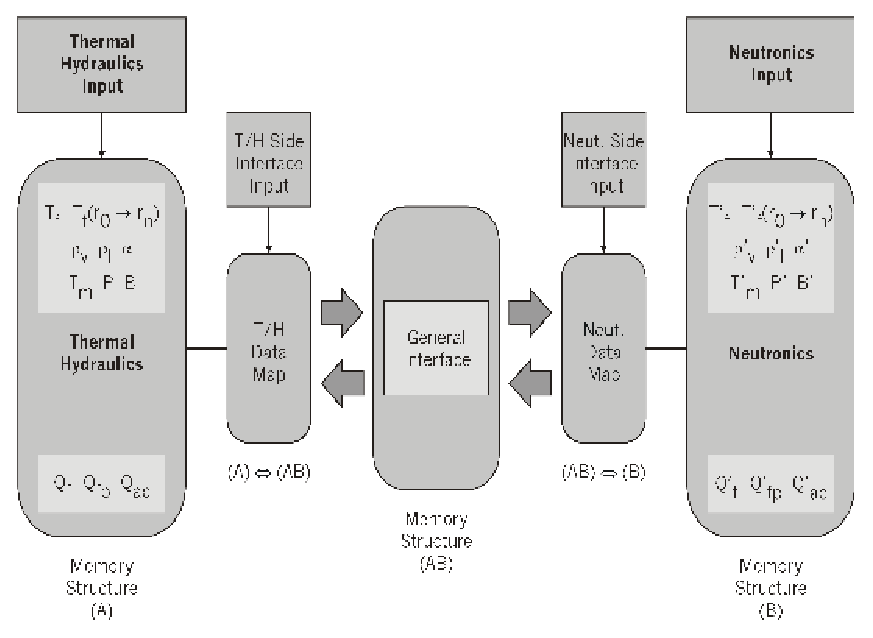
\includegraphics[scale=0.5]{pics/PARCS_coupling}
\par\end{centering}

\caption{PARCS Coupling Structure}


\label{fig:PARCSCoupling}
\end{figure}


After a steady state coupled solution is found, the time-dependent
solution can be calculated. In PARCS, this is done by an operator-split,
explicit scheme as shown in Fig. \ref{fig:PARCSTime}. In their time-marching
algorithm, the neutronics and thermal hydraulics are not converged
in a given time step. Although this is an approximation, it has shown
to be effective. 
\begin{figure}
\begin{centering}
%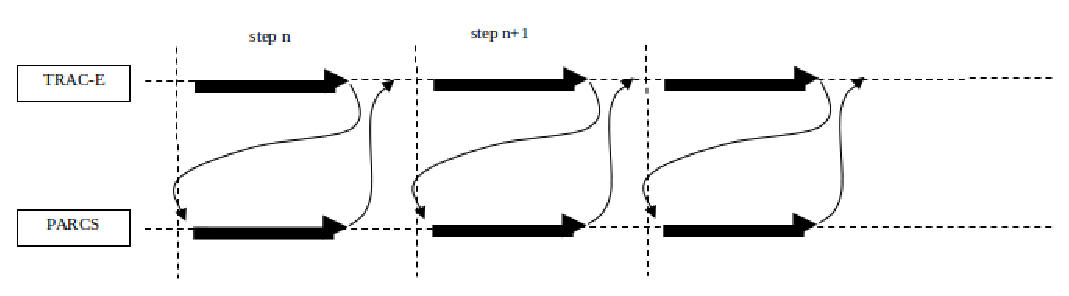
\includegraphics[scale=0.5]{pics/parcs_time}
\begin{tikzpicture}

	% Define background color
	\colorlet{bgcolor}{mitgray!20};

	% Define Dimensions
	\def\blockwidth{2.75cm};
	\def\blockheight{1.5cm};
	\def\elemheight{1cm};
	\def\elemwidth{2cm};
	\def\elemvsep{0.5cm};
	\def\elemhsep{0.75cm};
	
	% Define Outer Frame
	\tikzstyle{frame} = [rounded corners, fill=bgcolor, draw=black, double, very thick];
	\draw[frame] (0.0,0.0) rectangle (4*\blockwidth+0.1cm,2*\blockheight+0.5cm);

	% Define Elements in Frame
	\begin{scope}
		\tikzstyle{element} = [rectangle, rounded corners, draw = black, very thick, minimum height=\elemheight, minimum width=\elemwidth];	
		\node[element] (time 1t) at (0.5*\elemwidth+0.5*\elemhsep,0.5*\elemheight+0.5*\elemvsep) {T/H};
		\node[element,above = \elemvsep of time 1t.north] (time 1n) {Neutronics};
		\node[element,right = \elemhsep of time 1t.east] (time 2t) {T/H};
		\node[element,above = \elemvsep of time 2t.north] (time 2n) {Neutronics};
		\node[element,right = \elemhsep of time 2t.east] (time 3t) {T/H};
		\node[element,above = \elemvsep of time 3t.north] (time 3n) {Neutronics};
		\node[element,right = \elemhsep of time 3t.east] (time 4t) {T/H};
		\node[element,above = \elemvsep of time 4t.north] (time 4n) {Neutronics};
	\end{scope}
		
	% Draw connectors between elements
	\tikzstyle{connector} = [->, >=stealth, thick, shorten >=2pt];
	\draw[connector] (time 1n) to [out=270,in=90] (time 1t);
	\draw[connector] (time 1t) to [out=0,in=180]  (time 2n);
	\draw[connector] (time 2n) to [out=270,in=90] (time 2t);
	\draw[connector] (time 2t) to [out=0,in=180]  (time 3n);
	\draw[connector] (time 3n) to [out=270,in=90] (time 3t);
	\draw[connector,dashed] (time 3t) to [out=0,in=180]  (time 4n);
	\draw[connector] (time 4n) to [out=270,in=90] (time 4t);
	
	% Put labels in
	\tikzstyle{labels}    = [minimum height = 1.0cm, text centered, anchor = south];
	\node[labels,above = 0.4cm of time 1n.center] {$t=0$};
	\node[labels,above = 0.4cm of time 2n.center] {$t=\Delta t$};
	\node[labels,above = 0.4cm of time 3n.center] {$t=2\Delta t$};
	\node[labels,above = 0.4cm of time 4n.center] {$t=n\Delta t$};

\end{tikzpicture}
\par\end{centering}

\caption{PARCS Coupling Structure}


\label{fig:PARCSTime}
\end{figure}


In this paper, a fully coupled time-dependent solution between neutronics
and thermal hydraulics is performed. In this method, no operator splitting
is performed and the equations are solved non-linearly at the same
time. For this nonlinear system of equations, a Jacobian-Free Newton
Krylov (JFNK) method is applied.


\section{Model and Governing Equations}

\label{sec:Governing}In this section, the reactor model will be discussed
along with the governing equations that will be used to solve for
physics. For the geometry, a one-dimensional slab reactor is assumed.
A diagram of this model is shown in Fig. \ref{fig:geometry}. 
\begin{figure}
\begin{centering}
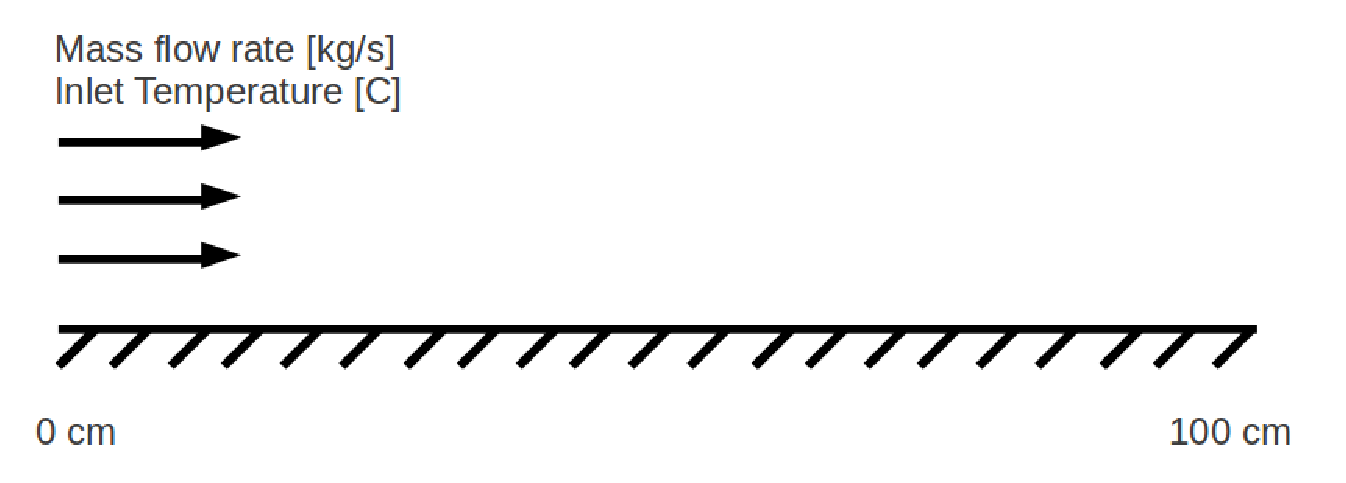
\includegraphics[scale=0.4]{pics/geometry}
\par\end{centering}

\caption{Geometry of Reactor Slab}


\label{fig:geometry}
\end{figure}
 In this geometry, the slab reactor (similar to modeling the axial
direction of a fuel pin) is assumed to be 370 cm. To remove the heat
produced from fission reactors in the core, a fluid is passed over
the slab. Here, only one dimensional flow is considered and only the
energy equation is applied since the flow rate will be specified and
remains constant. In addition, it will be assumed that the heat from
the reactor is completely dumped into the coolant and there is no
time constant for this process. Therefore, conduction and convective
heat transfer equations are not applied. With these assumptions, the
system of equations that remains is the simplest for these coupled
physics. This is important since the JFNK nonlinear algorithm is of
interest in this work.


\subsection{Neutron Diffusion Equation}

In this section, the governing equations to model the neutronics will
be presented. The neutron transport equation is the most detailed
form to describe the behavior how neutrons travel and interact in
a medium. In time-dependent form, the neutron transport equation is
\cite{Hebert2009}

\begin{equation}
\underbrace{\frac{1}{v}\frac{\partial\varphi}{\partial t}}_{\mathrm{time-dependent}}+\underbrace{\mathbf{\Omega}\cdot\nabla\varphi\left(\mathbf{r},E,\mathbf{\Omega},t\right)}_{\mathrm{neutron\, leakage}}+\underbrace{\Sigma_{t}\left(\mathbf{r},E,t\right)\varphi\left(\mathbf{r},E,\mathbf{\Omega},t\right)}_{\mathrm{interation\, of\, neutrons\, with\, medium}}=\underbrace{Q\left(\mathbf{r},E,\mathbf{\Omega},t\right)}_{\mathrm{neutron\, source}},\label{eq:FluxTransport}
\end{equation}
 
\begin{eqnarray}
Q\left(\mathbf{r},E,\mathbf{\Omega},t\right) & = & \underbrace{\int_{4\pi}d^{2}\Omega^{\prime}\int_{0}^{\infty}dE^{\prime}\Sigma_{s}\left(\mathbf{r},E^{\prime}\rightarrow E,\mathbf{\Omega}^{\prime}\rightarrow\mathbf{\Omega},t\right)\varphi\left(\mathbf{r},E^{\prime},\mathbf{\Omega}^{\prime},t\right)}_{\mathrm{neutrons\, scattering\, into\, phase\, space}}\label{eq:TransportSource}\\
 & + & \underbrace{\frac{1}{4\pi}\frac{\left(1-\beta\right)}{k_{eff}}\int_{0}^{\infty}dE^{\prime}\nu\Sigma_{f}\left(\mathbf{r},E^{\prime}\rightarrow Et\right)\varphi\left(\mathbf{r},E^{\prime},\mathbf{\Omega}^{\prime},t\right)}_{\mathrm{neutrons\, from\, prompt\, fissions}}+\underbrace{\frac{1}{4\pi}\sum_{l}\lambda_{d,l}c_{l}\left(\mathbf{r},t\right)}_{\mathrm{neutrons\, from\, precursor\, decay}}.\nonumber 
\end{eqnarray}
 The variables in these formulas are as follows:
\begin{itemize}
\item $v$ - neutron speed
\item $\varphi$ - angular neutron flux 
\item $t$ - time
\item $\mathbf{\Omega}$ - unit vector of neutron travel
\item $\mathbf{r}$ - spatial location of neutron
\item $E$ - neutron energy
\item $\Sigma_{t}$ - total macroscopic cross section
\item $Q$ - neutron source
\item $\Sigma_{s}$ - scattering macroscopic cross section
\item $\beta$ - total delayed neutron fraction
\item $\nu\Sigma_{f}$ - neutron fission production macroscopic cross section
\item $\lambda_{d,l}$ - delayed neutron precursor decay constant with subscript
$l$ for precursor group number
\item $c_{l}$ - delayed neutron precursor concentration
\item $k_{eff}$ - core multiplication factor
\end{itemize}
An important concept in reactor physics is $k_{eff}$ or the core
multiplication factor. In modeling of reactors, if the steady state
calculation is not perfectly balanced, neutron destruction does not
equal neutron production, and an eigenvalue is introduced to state
how far away from {}``steady'' the reactor is. If $k_{eff}$ is
unity then the neutron population is perfectly balanced. Therefore,
when beginning a transient calculation, for example with the equations
above, $k_{eff}$ from the steady state calculations must be used. 

To model the concentration of precursors the following equation is
used for each precursor group $l$, which describes a balance of precursor
production from fission reactions to their destruction from decay,

\begin{equation}
\frac{\partial c_{l}}{\partial t}=\underbrace{\frac{\beta}{k_{eff}}\int_{0}^{\infty}dE\int_{0}^{\infty}dE^{\prime}\nu\Sigma_{f}\left(\mathbf{r},E^{\prime}\rightarrow Et\right)\varphi\left(\mathbf{r},E^{\prime},\mathbf{\Omega}^{\prime},t\right)}_{\mathrm{neutrons\, from\, precursor\, decay}}-\underbrace{\lambda_{d,l}c_{l}\left(\mathbf{r},t\right)}_{\mathrm{precursor\, decay}}.\label{eq:TransportPrec}
\end{equation}
The assumption is that the decay of one precursor isotope will give
off one neutron. This is why the decay term shows up as a source of
neutrons in the neutron balance equation. From these transport equations,
the neutron diffusion equation can be derived. The form can be determined
by expanding the angular flux and scattering source in Legendre polynomials
and truncating after order 1. After the expansion and reduction, two
equations result. The first represents neutron balance and the other
is an equation that resembles Fick's Law (hence diffusion). They are
\begin{multline}
\frac{1}{v}\frac{\partial\phi}{\partial t}+\nabla\cdot\mathbf{J}\left(\mathbf{r},E,t\right)+\Sigma_{t}\left(\mathbf{r},E,t\right)\phi\left(\mathbf{r},E,t\right)=\\
\int_{0}^{\infty}dE^{\prime}\left[\Sigma_{s}\left(\mathbf{r},E^{\prime}\rightarrow E,t\right)+\frac{1-\beta}{k_{eff}}\nu\Sigma_{f}\left(\mathbf{r},E^{\prime}\rightarrow E,t\right)\right]\phi\left(\mathbf{r},E^{\prime},t\right)+\sum_{l}\lambda_{d,l}c_{l}\left(\mathbf{r},t\right),\label{eq:DiffusionBalance-1}
\end{multline}
 
\begin{equation}
\mathbf{J}\left(\mathbf{r},E,t\right)=-D\left(\mathbf{r},E,t\right)\nabla\phi\left(\mathbf{r},E,t\right).\label{eq:DiffusionFicks}
\end{equation}
 The equation to model the precursor cursor concentration is 

\begin{equation}
\frac{\partial c_{l}}{\partial t}=\frac{\beta}{k_{eff}}\int_{0}^{\infty}dE\int_{0}^{\infty}dE^{\prime}\nu\Sigma_{f}\left(\mathbf{r},E^{\prime}\rightarrow E,t\right)\phi\left(\mathbf{r},E^{\prime},t\right)-\lambda_{d,l}c_{l}\left(\mathbf{r},t\right).\label{eq:DiffusionPrec}
\end{equation}
 The new variables introduced here are
\begin{itemize}
\item $\phi$ - scalar neutron flux, $\phi=\int_{4\pi}\varphi d^{2}\Omega$
\item $\mathbf{J}$ - scalar neutron current, $\mathbf{J}=\int_{4\pi}\mathbf{\Omega}\varphi d^{2}\Omega$ 
\item $D$ - neutron diffusion coefficient
\end{itemize}

\subsubsection{One-dimensional One-group Transient Neutron Diffusion Equation}

For this paper, only the one-dimensional one-energy group transient
neutron diffusion equation is required. If Eq. (\ref{eq:DiffusionBalance-1})
is integrated over all energies and only 1 precursor group is considered,
the equations become
\begin{gather}
\frac{1}{v}\frac{\partial\phi}{\partial t}+\nabla\cdot\mathbf{J}\left(\mathbf{r},t\right)+\Sigma_{a}\left(\mathbf{r},t\right)\phi\left(\mathbf{r},t\right)=\frac{1-\beta}{k_{eff}}\nu\Sigma_{f}\left(\mathbf{r},t\right)\phi\left(\mathbf{r},t\right)+\lambda_{d}c\left(\mathbf{r},t\right),\label{eq:DiffusionBalance1g}
\end{gather}


\begin{equation}
\mathbf{J}\left(\mathbf{r},t\right)=-D\left(\mathbf{r},t\right)\nabla\phi\left(\mathbf{r},t\right),\label{eq:DiffusionFicks1g}
\end{equation}
 
\begin{equation}
\frac{\partial c}{\partial t}=\frac{\beta}{k_{eff}}\nu\Sigma_{f}\left(\mathbf{r},t\right)\phi\left(\mathbf{r},t\right)-\lambda_{d}c\left(\mathbf{r},t\right).\label{eq:DiffusionPrec1g}
\end{equation}
 In Eq. (\ref{eq:DiffusionBalance1g}), the neutron absorption macroscopic
cross section is introduced. This cross section is defined as the
difference between the total and scattering macroscopic cross section,
$\Sigma_{a}\equiv\Sigma_{t}-\Sigma_{s}$. The equations can be further
reduced to 1-dimension and become

\begin{equation}
\frac{1}{v}\frac{\partial\phi}{\partial t}+\frac{\partial J}{\partial x}+\Sigma_{a}\left(x,t\right)\phi\left(x,t\right)=\frac{1-\beta}{k_{eff}}\nu\Sigma_{f}\left(x,t\right)\phi\left(x,t\right)+\lambda_{d}c\left(x,t\right),\label{eq:Diffusion1g1d}
\end{equation}
 
\begin{equation}
J\left(x,t\right)=-D\left(x,t\right)\frac{\partial\phi}{\partial x},\label{eq:DiffusionFicks1g1d}
\end{equation}
 
\begin{equation}
\frac{\partial c}{\partial t}=\frac{\beta}{k_{eff}}\nu\Sigma_{f}\left(x,t\right)\phi\left(x,t\right)-\lambda_{d}c\left(x,t\right).\label{eq:DiffusionPrec1d1g}
\end{equation}
 Equations (\ref{eq:Diffusion1g1d}), (\ref{eq:DiffusionFicks1g1d})
and (\ref{eq:DiffusionPrec1d1g}) form the set of transient neutronics
equations that will be solved in this paper. 


\subsubsection{Steady State Form of the Neutron Diffusion Equation}

Equations (\ref{eq:Diffusion1g1d}), (\ref{eq:DiffusionFicks1g1d})
and (\ref{eq:DiffusionPrec1d1g}) can be reduced to steady by removing
the time-derivative term. This is shown as

\begin{equation}
\frac{dJ}{dx}+\Sigma_{a}\left(x\right)\phi\left(x\right)=\frac{1-\beta}{k_{eff}}\nu\Sigma_{f}\left(x\right)\phi\left(x\right)+\lambda_{d}c\left(x\right),\label{eq:DiffusionBalSteady}
\end{equation}
 
\begin{equation}
J\left(x\right)=-D\left(x\right)\frac{d\phi}{dx},\label{eq:DiffusionFicksSteady}
\end{equation}
\begin{equation}
\lambda_{d}c\left(x\right)=\frac{\beta}{k_{eff}}\nu\Sigma_{f}\left(x\right)\phi\left(x\right).\label{eq:DiffusionPrecSteady}
\end{equation}
 Equation (\ref{eq:DiffusionPrecSteady}) can be combined with Eq.
(\ref{eq:DiffusionBalSteady}) to give the final form of the 1-D neutron
balance equation,
\begin{equation}
\frac{dJ}{dx}+\Sigma_{a}\left(x\right)\phi\left(x\right)=\frac{1}{k_{eff}}\nu\Sigma_{f}\left(x\right)\phi\left(x\right).\label{eq:DiffusionSteady}
\end{equation}
Note that Eq. (\ref{eq:DiffusionSteady}) is an eigenvalue problem
since neutron current depends on flux through Fick's law. Here the
spatial flux distribution represents the eigenfunction and $1/k_{eff}$
is the eigenvalue which is commonly denoted as $\lambda$ (not to
be confused with the decay constant, $\lambda_{d}$). 


\subsection{Coupling Neutrons to Thermal Hydraulics }

From the steady state neutronic analysis a neutron flux distribution
is obtained. Since the flux is an eigenfunction, it must be normalized
to some physical quantity to have meaning. In reactor physics the
flux is normalized to reactor power. This step is known as flux-to-power
normalization. This step can be calculated by computing the energy
per fission multiplied by the fission reaction rate and integrated
over all space and volume. This is represented mathematically as 
\begin{equation}
Q_{r}=\tilde{c}\int_{V}d^{3}r\int_{0}^{\infty}dE\kappa\Sigma_{f}\left(\mathbf{r},E\right)\phi\left(\mathbf{r},E\right).
\end{equation}
Here, the variables are
\begin{itemize}
\item $Q_{r}$ - reactor power
\item $\tilde{c}$ - flux-to-power normalization constant
\item $\kappa\Sigma_{f}$ - energy (from fission) deposition cross section
\end{itemize}
In one dimension and one energy group this is
\begin{equation}
Q_{R}=\tilde{c}\int_{0}^{L}dx\kappa\Sigma_{f}\left(x\right)\phi\left(x\right).\label{eq:fluxpownorm}
\end{equation}
Note that this step only needs to be performed during the steady state
analysis since the transient analysis is not an eigenvalue problem.
The transient equations are given the eigenvalue and eigenvector normalization
constant and these parameters are held constant throughout the transient. 

Once this normalization constant is determined from the steady state
calculation, the time-dependent spatial distribution of power density,
$Q\left(x,t\right)$ can be calculated as

\begin{equation}
Q\left(x,t\right)=\tilde{c}\kappa\Sigma_{f}\left(x,t\right)\phi\left(x,t\right).\label{eq:energydep}
\end{equation}
 This can be reduced to steady state to give

\begin{equation}
Q\left(x\right)=\tilde{c}\kappa\Sigma_{f}\left(x\right)\phi\left(x\right).\label{eq:energydepSteady}
\end{equation}
 


\subsection{Thermal Hydrualics - Energy Equation}

The energy equation for a single phase fluid is given by \cite{Todreas2011}

\begin{equation}
\frac{\partial\left(\rho h\right)}{\partial t}+\nabla\cdot\left(\rho h\mathbf{u}\right)=-\nabla\cdot\mathbf{q}^{\prime\prime}+q^{\prime\prime\prime}+\frac{Dp}{Dt}+\Phi.\label{eq:EnergyFull}
\end{equation}
 The variables in this equation are
\begin{itemize}
\item $\rho$ - density of fluid
\item $h$ - enthalpy of fluid
\item t - time
\item \textbf{$\mathbf{u}$ }- velocity vector
\item $\mathbf{q}^{\prime\prime}$ - heat flux vector
\item $q^{\prime\prime\prime}$ - volumetric heat source
\item $p$ - pressure
\item $\Phi$ - dissipation function
\end{itemize}
Assuming inviscid flow, the energy equation reduces to 

\begin{equation}
\frac{\partial\left(\rho h\right)}{\partial t}+\nabla\cdot\left(\rho h\mathbf{u}\right)=-\nabla\cdot\mathbf{q}^{\prime\prime}+q^{\prime\prime\prime}.\label{eq:energyinviscid}
\end{equation}
 Assuming one-dimensional flow and no heat flux, the energy becomes

\begin{equation}
\frac{\partial\left(\rho h\right)}{\partial t}+\frac{\partial\left(\rho hu\right)}{\partial x}=q^{\prime\prime\prime}.
\end{equation}
It will be assumed that the energy produced from fissions will be
a volumetric heat source in the energy equation (note this is not
common since fissions occur in fuel and not in coolant). Multiplying
this form of the energy equation by the {}``area'', $A$, of the
flow, it can be rewritten as follows

\begin{equation}
A\frac{\partial\left(\rho h\right)}{\partial t}+w\frac{\partial h}{\partial x}=q^{\prime}.
\end{equation}
 The new variables that appear in the above equation are
\begin{itemize}
\item $w$ - mass flow rate calculated as $w=\rho uA$ which from the continuity
equation must be constant spatially and therefore taken out of the
differential
\item $q^{\prime}$ - linear heat rate calculated as $q^{\prime}=q^{\prime\prime\prime}A$ 
\end{itemize}
If the variation of density from thermal expansion is neglected as
a function of time the equation reduces to 

\begin{equation}
\rho A\frac{\partial h}{\partial t}+w\frac{\partial h}{\partial x}=q^{\prime}.
\end{equation}
 Using the constitutive relation between enthalpy and temperature
for an incompressible fluid that $dh=c_{p}dT$, the energy equation
becomes

\begin{equation}
\rho Ac_{p}\frac{\partial T}{\partial t}+wc_{p}\frac{\partial T}{\partial x}=q^{\prime}.\label{eq:energy1DTrans}
\end{equation}
 This is the transient form of the energy equation that is solved
in this paper. For steady state, the energy equation becomes 
\begin{equation}
wc_{p}\frac{dT}{dx}=q^{\prime}.\label{eq:energy1D}
\end{equation}
 Note that if the energy equation is integrated over the whole reactor,
the outlet temperature can be calculated with

\begin{equation}
T_{out}=T_{in}+\frac{Q_{r}}{wc_{p}}.
\end{equation}
 


\subsection{Thermal Hydraulic to Neutronic Coupling}

The macroscopic cross sections and diffusion coefficient that were
described in the neutronics formulation depend on density of the coolant.
This is due to the fact that besides water functioning as a coolant
in a nuclear reactor, it has the dual purpose of also slowing down
neutrons. Slow neutrons have a higher probability of causing a fission
reaction. This process is almost analogous to billiard ball elastic
collisions. Thus, if the density of water is low, it is less effective
at slowing down neutrons and will have a negative effect the rate
at which fissions occur. This is why nuclear reactors are somewhat
self-regulating. If the power suddenly increases in a region of the
core, the temperature will increase lowering the density and thus
decreasing the fission rate and power. Note that this may not be the
dominant effect as there are other nuclear process that will also
have a negative effect on the fission rate such as fuel temperature.
In this paper, only the effect of density is modeled. 

Once the temperature distribution is known, the density distribution
can be calculated from the equation of state for water as the pressure
is specified. Thus, 

\begin{equation}
\rho\left(x,t\right)=\rho\left(T\left(x,t\right),p\right).\label{eq:StateEq}
\end{equation}
The state equation is evaluated in the X-Steam look-up tables for
MATLAB \cite{Holmgren2006}. Since the macroscopic cross sections
and diffusion coefficient are to first order linear with density,
the following formulas can be used to describe the dependence of these
neutronic parameters on density:

\begin{equation}
\Sigma_{a}\left(x,t\right)=\Sigma_{a}^{ref}+\frac{\partial\Sigma_{a}}{\partial\rho}\left[\rho\left(x,t\right)-\rho^{ref}\right],\label{eq:AbsRHO}
\end{equation}


\begin{equation}
\nu\Sigma_{f}\left(x,t\right)=\nu\Sigma_{f}^{ref}+\frac{\partial\nu\Sigma_{f}}{\partial\rho}\left[\rho\left(x,t\right)-\rho^{ref}\right],\label{eq:NfissRHO}
\end{equation}


\begin{equation}
D\left(x,t\right)=D^{ref}+\frac{\partial D}{\partial\rho}\left[\rho\left(x,t\right)-\rho^{ref}\right],\label{eq:DiffRHO}
\end{equation}
 

\begin{equation}
\kappa\Sigma_{f}\left(x,t\right)=\kappa\Sigma_{f}^{ref}+\frac{\partial\kappa\Sigma_{f}}{\partial\rho}\left[\rho\left(x,t\right)-\rho^{ref}\right].\label{eq:KfissRHO}
\end{equation}
 For each of the above equations, there is a reference value and are
described in Section \pageref{sub:Reference}. 


\subsection{Calculation of Reference Neutronic Parameters }

\label{sub:Reference}To calculate macroscopic cross sections and
diffusion coefficients for core simulation, the 2-D neutron transport
equation is solved. To solve this complicated PDE in space angle and
energy, a stochastic Monte Carlo code, Serpent, is used to generate
these parameters \cite{LeppanenUser2010}. For this calculation a
typical nuclear fuel rod is used depicted in Fig. \ref{fig:pincell}.
\begin{figure}
\begin{centering}
\includegraphics[scale=0.15]{pics/pincell_serp_geom1}
\par\end{centering}

\caption{Typical 2-D Cross Section of a Fuel Rod}


\label{fig:pincell}
\end{figure}
 

For the Seabrook Nuclear Reactor, the inlet temperature the core is
$293.1\,\mathrm{^{\circ}C}$ and the outlet temperature is $326.8\,\mathrm{^{\circ}C}$.
The core average temperature is taken as the straight average of these
two values to give

\[
T^{ref}=310\,\mathrm{^{\circ}C}.
\]
 The pressure of the Seabrook nuclear reactor is $155$ bar. Therefore
using XSteam, the density of water at this pressure and average temperature
is 
\[
\rho^{ref}=0.705\,\mathrm{g/cc}.
\]
 The input file for the Serpent code with these reference conditions
is listed in Appendix . The reference neutronic parameters from the
Serpent code (neglecting their associated uncertainties from the stochastic
process) are as follows:

\[
\Sigma_{a}^{ref}=2.27516\times10^{-2}\,\mathrm{cm^{-1}},
\]


\[
\nu\Sigma_{f}^{ref}=3.13791\times10^{-2}\,\mathrm{cm^{-1}},
\]


\[
D^{ref}=8.85342\times10^{-1}\,\mathrm{cm},
\]


\[
\kappa\Sigma_{f}^{ref}=4.13494\times10^{-13}\,\mathrm{cm^{-1}}.
\]
Perturbations of -10\%, -5\%, +5\% and +10\% were made to the reference
density to obtain the dependence of the above parameters on density.
These points are then fit with a linear regression to determine the
slope of the data. This regression was performed for each of the parameters
above and plots of this regression is shown in Figs. \ref{fig:absxsRHO}-\ref{fig:kfissRHO}.
\begin{figure}
\begin{centering}
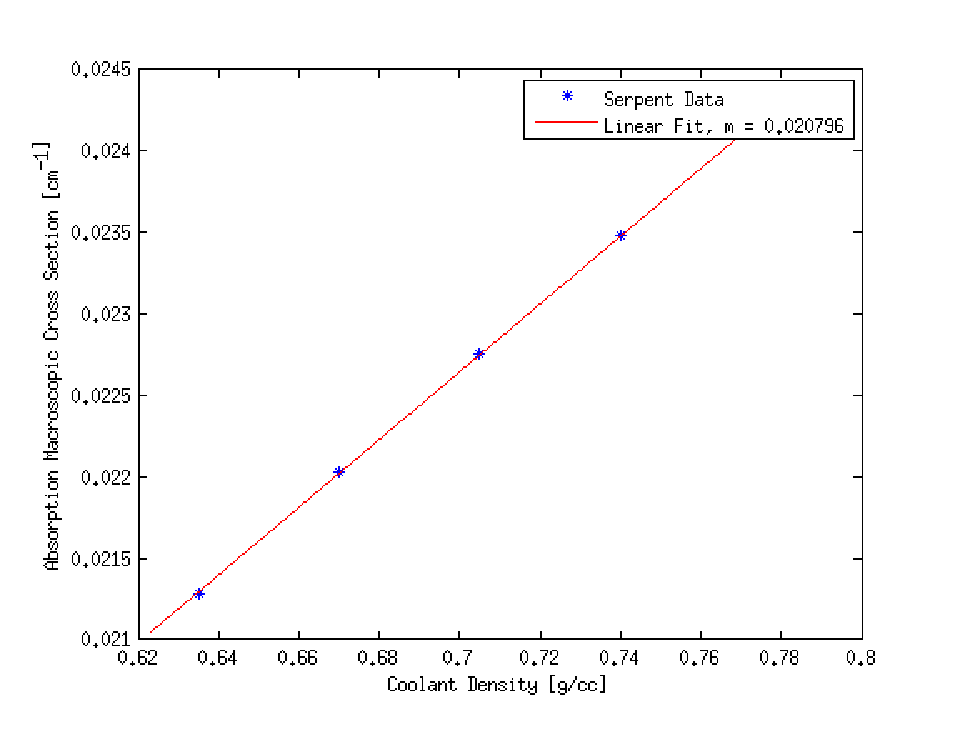
\includegraphics[scale=0.7]{pics/absxs}
\par\end{centering}

\caption{Dependence of Absorption Macroscopic Cross Section on Density}


\label{fig:absxsRHO}
\end{figure}
 
\begin{figure}
\begin{centering}
\includegraphics[scale=0.7]{pics/nfiss}
\par\end{centering}

\caption{Dependence of Fission Neutron Production Macroscopic Cross Section
on Density}


\label{fig:nfissRHO}
\end{figure}
 
\begin{figure}
\begin{centering}
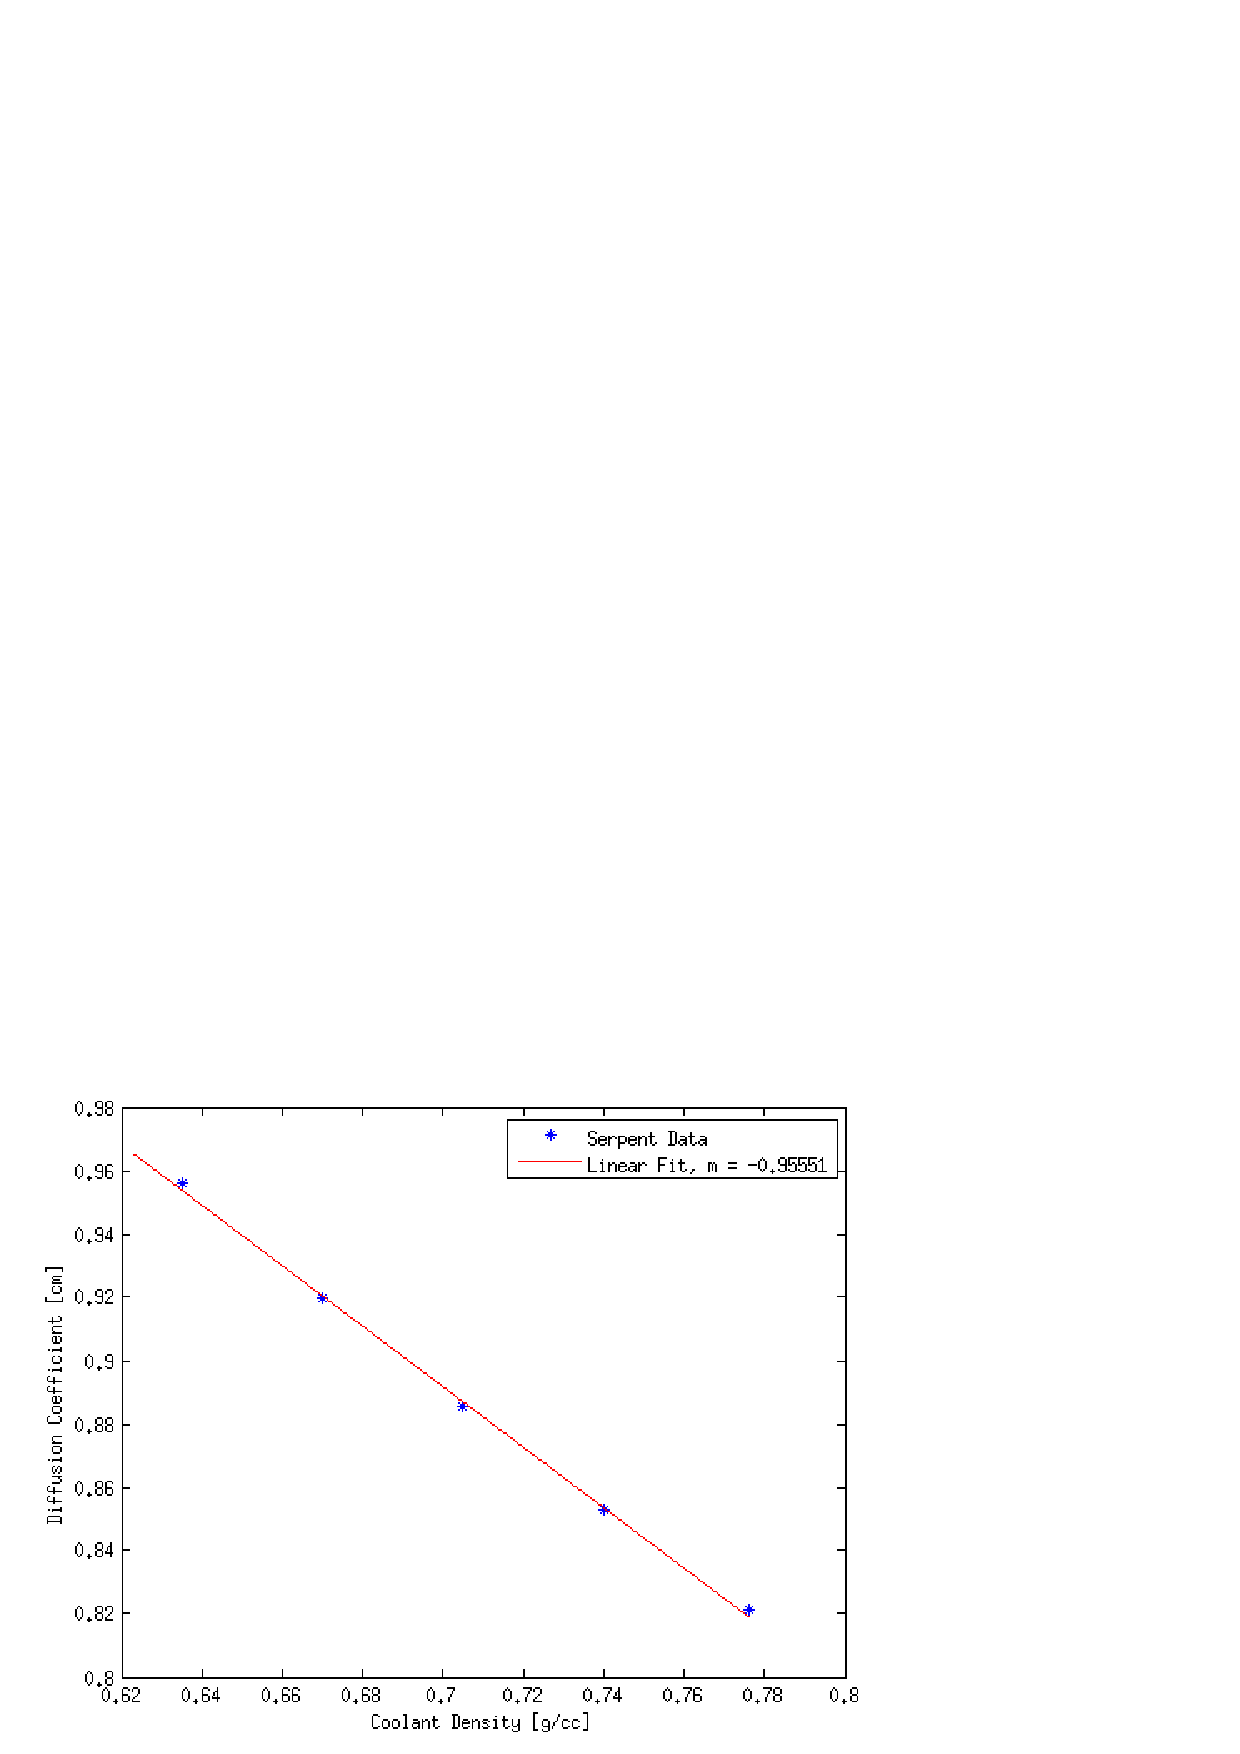
\includegraphics[scale=0.7]{pics/diff}
\par\end{centering}

\caption{Dependence of Diffusion Coefficient on Density}


\label{fig:diffRHO}
\end{figure}
 
\begin{figure}
\begin{centering}
\includegraphics[scale=0.7]{pics/kfiss}
\par\end{centering}

\caption{Dependence of Energy Deposition Macroscopic Cross Section on Density}


\label{fig:kfissRHO}
\end{figure}
 From each of the figures, it can be observed that the trend of the
data is linear. The slopes of the regressions are as follows:

\[
\frac{\partial\Sigma_{a}}{\partial\rho}=0.020796,
\]
 
\[
\frac{\partial\nu\Sigma_{f}}{\partial\rho}=0.035471,
\]
 
\[
\frac{\partial D}{\partial\rho}=-0.95551,
\]
 
\[
\frac{\partial\kappa\Sigma_{f}}{\partial\rho}=4.7055\times10^{-13}.
\]
From the results the macroscopic cross sections have a positive slope
while the diffusion coefficient has a negative slope. The cross section
dependence makes sense since as the density increases, neutrons will
slow down more and cause more fission. The opposite is true for the
diffusion coefficient, if the density increases, neutrons are more
efficiently slowed down in and therefore will not diffuse as much.
Therefore, if the density goes down there will be a negative effect
on producing more neutrons from fission as the cross section will
go down and neutrons will diffuse further and have a higher probability
of leaking out of the core.


\section{Discretization of Equations}

In this section, the governing 1-D equations presented in Section
\ref{sec:Governing} are discretized in space and time. Before a transient
calculation can be performed, a steady solution must be determined.
Therefore, the discretization of the steady state form of the equations
will be presented first. It is assumed that the grid is discretized
uniformly over the slab.


\subsection{Steady-State Equations}

For the discretization in space, a second order finite volume method
will be used. This discretization is shown in Fig. \ref{fig:discretization}.
\begin{figure}
\begin{centering}
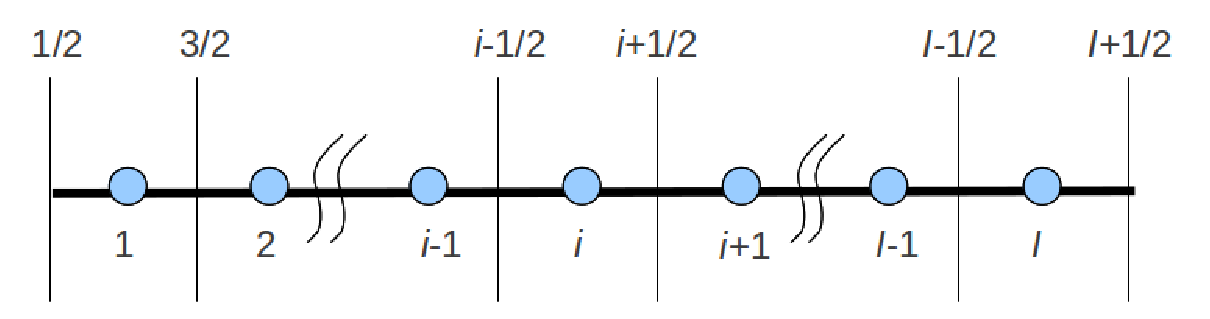
\includegraphics[scale=0.5]{pics/discretizaton}
\par\end{centering}

\caption{Spatial Discretization of 1-D Geometry}


\label{fig:discretization}
\end{figure}



\subsubsection{Neutronics}

\label{sub:SteadyNeut}

We can integrate each term in Eq. (\ref{eq:DiffusionSteady}) over
cell $i$,

\begin{equation}
\int_{x_{i-1/2}}^{x_{i+1/2}}dx\frac{dJ}{dx}+\int_{x_{i-1/2}}^{x_{i+1/2}}dx\Sigma_{a}\left(x\right)\phi\left(x\right)=\int_{x_{i-1/2}}^{x_{i+1/2}}dx\frac{1}{k_{eff}}\nu\Sigma_{f}\left(x\right)\phi\left(x\right).
\end{equation}
 The average flux in cell $i$ can be calculated as

\begin{equation}
\bar{\phi}_{i}=\frac{1}{\Delta x}\int_{x_{i-1/2}}^{x_{i+1/2}}dx\phi\left(x\right).
\end{equation}
 The average flux is for cell $i$ is then taken to be the value at
the center of the cell,

\begin{equation}
\bar{\phi}_{i}=\bar{\phi}_{i}\left(x_{i}\right)=\phi\left(x_{i}\right)+O\left(\Delta x^{2}\right).
\end{equation}
 This is a second order approximation. It is also assumed in this
derivation that neutronic parameters are spatially constant in a cell.
Performing the integration over cell $i$, the neutron balance equation
becomes

\begin{equation}
J_{i+1/2}-J_{i-1/2}+\Sigma_{a,i}\bar{\phi}_{i}\Delta x=\frac{1}{k_{eff}}\nu\Sigma_{f,i}\bar{\phi}_{i}\Delta x.\label{eq:FVNeutBalance}
\end{equation}
 The fluxes that show up in finite volume equations are actually the
neutron current, NOT the neutron flux. From Fick's Law in Eq. (\ref{eq:DiffusionFicksSteady}),
the fluxes at the surfaces of the mesh cell are given by 

\begin{equation}
J_{i+1/2}=-D_{i}\left.\frac{d\phi}{dx}\right|_{i+1/2}\qquad J_{i-1/2}=-D_{i}\left.\frac{d\phi}{dx}\right|_{i-1/2}.
\end{equation}
 A second order central difference scheme is applied to approximate
the derivative of the flux at the boundary. Since the diffusion coefficients
in adjacent cells do not necessarily need to be constant, the current
at the interface between adjacent cells must be equivalent. For the
$i+1/2$ interface, the current from the left cell is equated to the
current from the right cell,

\begin{equation}
-D_{i}\left.\frac{d\phi}{dx}\right|_{i+1/2}=-D_{i+1}\left.\frac{d\phi}{dx}\right|_{i+1/2}.
\end{equation}
Applying a second order finite difference to the derivatives, the
current continuity becomes
\begin{equation}
-D_{i}\frac{\phi_{i+1/2}-\bar{\phi}_{i}}{\Delta x/2}=-D_{i+1}\frac{\bar{\phi}_{i+1}-\phi_{i+1/2}}{\Delta x/2}.
\end{equation}
 The flux at the interface can be represented as

\begin{equation}
\phi_{i+1/2}=\frac{2}{\Delta x}\frac{D_{i+1}}{D_{i+1}+D_{i}}\left(\bar{\phi}_{i+1}-\bar{\phi}_{i}\right).
\end{equation}
 Therefore the current or finite volume flux at the right interface
is 

\begin{equation}
J_{i+1/2}=-\frac{2}{\Delta x}\frac{D_{i+1}D_{i}}{D_{i+1}+D_{i}}\left(\bar{\phi}_{i+1}-\bar{\phi}_{i}\right).
\end{equation}
 Notice that if the diffusion coefficient is equivalent in adjacent
cells, the equation reduces to the simple second order central difference.
Similarly for the left interface, the current is

\begin{equation}
J_{i-1/2}=-\frac{2}{\Delta x}\frac{D_{i}D_{i-1}}{D_{i}+D_{i-1}}\left(\bar{\phi}_{i}-\bar{\phi}_{i-1}\right).
\end{equation}
 Substituting these currents into Eq. (\ref{eq:FVNeutBalance}) the
discretized diffusion equation is

\begin{multline}
-\frac{2}{\Delta x}\frac{D_{i+1}D_{i}}{D_{i+1}+D_{i}}\left(\bar{\phi}_{i+1}-\bar{\phi}_{i}\right)+\frac{2}{\Delta x}\frac{D_{i}D_{i-1}}{D_{i}+D_{i-1}}\left(\bar{\phi}_{i}-\bar{\phi}_{i-1}\right)+\Sigma_{a,i}\bar{\phi}_{i}\Delta x=\frac{1}{k_{eff}}\nu\Sigma_{f,i}\bar{\phi}_{i}\Delta x.
\end{multline}
 Grouping like terms on the left hand side of the equation and dividing
by the cell volume, 

\begin{multline}
-\frac{2}{\Delta x^{2}}\frac{D_{i}D_{i-1}}{D_{i}+D_{i-1}}\bar{\phi}_{i-1}+\left(\frac{2}{\Delta x^{2}}\frac{D_{i+1}D_{i}}{D_{i+1}+D_{i}}+\frac{2}{\Delta x^{2}}\frac{D_{i}D_{i-1}}{D_{i}+D_{i-1}}+\Sigma_{a,i}\right)\bar{\phi}_{i}-\frac{2}{\Delta x^{2}}\frac{D_{i+1}D_{i}}{D_{i+1}+D_{i}}\bar{\phi}_{i+1}\\
=\frac{1}{k_{eff}}\nu\Sigma_{f,i}\bar{\phi}_{i}.\label{eq:IntNeut}
\end{multline}
 Since the neutron diffusion equation is a second order differential
equation, two boundary conditions must be specified. A physical boundary
condition is to say that once a neutron leaves the reactor it will
never come back. This may not always be true, especially depending
on how the boundaries are defined. Another neutronic parameter called
an albedo is defined as the ratio of incoming current of neutrons
at an interface to the outgoing current of neutrons,

\begin{equation}
\beta=\frac{J_{in}}{J_{out}}.\label{eq:albedo}
\end{equation}
 For the left boundary the current is 

\begin{equation}
J_{1/2}=-D_{1}\left.\frac{d\phi}{dx}\right|_{1/2}.\label{eq:Ficks1/2}
\end{equation}
 The current at an interface is actually the net neutron current at
that surface. This net current can always be decomposed into a partial
current going to the right and a partial current going to the left.
The relation between these partial currents to the net current is
represented as

\begin{equation}
J=J_{right}-J_{left}.\label{eq:Jleftright}
\end{equation}
 Current to the right is taken as positive since the positive $x$
direction is directed to the right as well. Notice that depending
on the boundary, the partial current to the right may be the same
as the incoming current or the outgoing current. For the left boundary,
the net current is 
\begin{equation}
J_{1/2}=J_{in}-J_{out}=-D_{1}\left.\frac{d\phi}{dx}\right|_{1/2}.\label{eq:Jinout}
\end{equation}
 From neutron transport theory, the partial incoming and outgoing
currents can be represent in terms of the flux at the boundary (Marshak
Boundary Conditions \cite{Bell1970}),
\begin{equation}
J_{left}=\frac{1}{4}\phi_{1/2}-\frac{1}{2}J_{1/2}\qquad J_{right}=\frac{1}{4}\phi_{1/2}+\frac{1}{2}J_{1/2}.\label{eq:Marshak}
\end{equation}
 Comparing Eqs. (\ref{eq:Jleftright}) and (\ref{eq:Jinout}), the
Marshak boundary conditions are

\[
J_{out}=\frac{1}{4}\phi_{1/2}-\frac{1}{2}J_{1/2}\qquad J_{in}=\frac{1}{4}\phi_{1/2}+\frac{1}{2}J_{1/2}.
\]
 These partial current equations can be substituted in to Eq. (\ref{eq:albedo})
and the net current can be determined to be

\begin{equation}
J_{1/2}=-\frac{1}{2}\frac{1-\beta}{1+\beta}\phi_{1/2}.
\end{equation}
 Substituting this expression into Eq. (\ref{eq:Ficks1/2}) and taking
a first order finite difference of the spatial derivative, Fick's
law becomes
\begin{equation}
-\frac{1}{2}\frac{1-\beta}{1+\beta}\phi_{1/2}=-D_{1}\frac{\bar{\phi}_{1}-\phi_{1/2}}{\Delta x/2}.
\end{equation}
 The surface flux at the left boundary is determined to be

\begin{equation}
\phi_{1/2}=\frac{4\left(1+\beta\right)D_{1}}{4D_{1}\left(1+\beta\right)+\Delta x\left(1-\beta\right)}\bar{\phi}_{1}.
\end{equation}
 Substituting this equation back into Eq. (\ref{eq:Ficks1/2}) after
applying the first order finite difference, the net current at the
boundary is 

\[
J_{1/2}=-\frac{2D_{1}\left(1-\beta\right)}{4D_{1}\left(1+\beta\right)+\Delta x\left(1-\beta\right)}\bar{\phi}_{1}.
\]
 Using the exact same process (except incoming/outgoing current definitions
switch) the net current on the right boundary is 

\[
J_{I+1/2}=\frac{2D_{I}\left(1-\beta\right)}{4D_{I}\left(1+\beta\right)+\Delta x\left(1-\beta\right)}\bar{\phi}_{I}.
\]
 The final form of the discretized equation for the left boundary
is 
\begin{multline}
\left(\frac{2}{\Delta x^{2}}\frac{D_{2}D_{1}}{D_{2}+D_{1}}+\frac{2}{\Delta x}\frac{\left(1-\beta\right)D_{1}}{4D_{1}\left(1+\beta\right)+\Delta x\left(1-\beta\right)}+\Sigma_{a,1}\right)\bar{\phi}_{1}\\
-\frac{2}{\Delta x^{2}}\frac{D_{2}D_{1}}{D_{2}+D_{1}}\bar{\phi}_{2}=\frac{1}{k_{eff}}\nu\Sigma_{f,1}\bar{\phi}_{1}.\label{eq:LeftNeut}
\end{multline}
 For the right boundary it is

\begin{multline}
-\frac{2}{\Delta x^{2}}\frac{D_{I}D_{I-1}}{D_{I}+D_{I-1}}\bar{\phi}_{I-1}+\left(\frac{2D_{I}\left(1-\beta\right)}{4D_{I}\left(1+\beta\right)+\Delta x\left(1-\beta\right)}+\frac{2}{\Delta x^{2}}\frac{D_{I}D_{I-1}}{D_{I}+D_{I-1}}+\Sigma_{a,I}\right)\bar{\phi}_{I}\\
=\frac{1}{k_{eff}}\nu\Sigma_{f,I}\bar{\phi}_{I}.\label{eq:RightNeut}
\end{multline}
 Equations (\ref{eq:IntNeut}), (\ref{eq:LeftNeut}) and (\ref{eq:RightNeut})
can be represented in matrix notation as

\begin{equation}
\mathbb{M}\bar{\mathbf{\Phi}}=\lambda\mathbb{F}\bar{\mathbf{\Phi}},\label{eq:NeutronOper}
\end{equation}
 where
\begin{itemize}
\item $\mathbb{M}$ is the neutron destruction operator,
\item $\bar{\mathbf{\Phi}}$ is a vector of cell average fluxes,
\item $\lambda$ is the eigenvalue of the system, which is $1/k_{eff}$,
\item $\mathbb{F}$ is the neutron production operator. 
\end{itemize}
The neutron destruction operator has a tridiagonal form while the
production operator is a diagonal of fission neutron production macroscopic
cross sections. Since this eigenvalue problem will be formulated in
a nonlinear sense, another equation is needed to constrain the eigenvector.
The common approach is to make the L2-norm of the eigenvector be unity
\cite{Gill2009},

\begin{equation}
\left\Vert \bar{\mathbf{\Phi}}\right\Vert _{2}=1.\label{eq:norm}
\end{equation}



\subsubsection{Coupling Neutrons to Thermal Hydraulics }

The normalization condition in Eq. (\ref{eq:fluxpownorm}) can be
converted into a summation of discrete volumes as

\begin{equation}
Q_{R}=\tilde{c}\int_{0}^{L}dx\kappa\Sigma_{f}\left(x\right)\phi\left(x\right)=\tilde{c}\sum_{i}\kappa\Sigma_{f,i}\bar{\phi}_{i}\Delta x=\tilde{c}\kappa\mathbf{\Sigma}_{f}^{\mathrm{T}}\bar{\mathbf{\Phi}}\Delta x.\label{eq:normfluxdiscrete}
\end{equation}
Once the normalization constant is determined the power in each volume
can be determined by integrating the power density,Eq. (\ref{eq:energydep}),
over a cell volume. The resulting formula is

\begin{equation}
Q_{i}=\int_{x_{i-1/2}}^{x_{i+1/2}}\tilde{c}\kappa\Sigma_{f}\phi\left(x\right)=\tilde{c}\kappa\Sigma_{f}\bar{\phi}_{i}\Delta x.\label{eq:powerdiscrete}
\end{equation}
In matrix form, the above equation is represented by

\begin{equation}
\mathbf{Q}=\tilde{c}\mathbb{E}\bar{\mathbf{\Phi}}\Delta x,\label{eq:energyoper}
\end{equation}
 the energy deposition operator $\mathbb{E}$ is a diagonal matrix
of the energy deposition cross section.


\subsubsection{Energy Equation}

The steady state energy can be integrated over cell $i$ to give

\begin{equation}
\int_{x_{i-1/2}}^{x_{i+1/2}}dx\frac{dT}{dx}=\int_{x_{i-1/2}}^{x_{i+1/2}}dx\frac{q^{\prime}}{wc_{p}}.
\end{equation}
After integration, 

\begin{equation}
T_{i+1/2}-T_{i-1/2}=\frac{Q_{i}}{wc_{p}}.\label{eq:FVEnergy}
\end{equation}
 We can define the average cell temperature and take it at the center
of the cell 
\begin{equation}
\bar{T}_{i}\approx\frac{1}{\Delta x}\int_{x_{i-1/2}}^{x_{i+1/2}}dxT\left(x\right).
\end{equation}
 The surface temperature on the left can be related to the temperature
in the left adjacent cell as

\begin{equation}
T_{i-1/2}=\bar{T}_{i-1}+\frac{Q_{i-1}}{2wc_{p}}
\end{equation}
 since only half of the energy is deposited between the center of
the cell and the surface. Similarly the right surface temperature
can be related to the cell average temperature as

\begin{equation}
T_{i+1/2}=\bar{T}_{i}+\frac{Q_{i}}{2wc_{p}}.
\end{equation}
 These two approximations are known as Upwind approximations. Substituting
these surface temperatures into Eq. (\ref{eq:FVEnergy}) to give a
relation between cell average temperatures
\begin{equation}
\bar{T}_{i}-\bar{T}_{i-1}=\frac{1}{2wc_{p}}Q_{i-1}+\frac{1}{2wc_{p}}Q_{i}.\label{eq:EnergyDiscret}
\end{equation}
 This can be represented in matrix notation as

\begin{equation}
\mathbb{S}\mathbf{\bar{T}}=\mathbb{R}\mathbf{Q},\label{eq:TempOper}
\end{equation}
 where $\mathbb{S}$ is the temperature operator and contains a diagonal
and a subdiagonal and $\mathbb{R}$ is the energy operator and is
comprised of a diagonal and subdiagonal. 


\subsubsection{Energy to Neutronic Coupling}

These coupling equations can very simply be converted for a whole
cell. The cell average density can be related to the cell average
density as

\begin{equation}
\rho_{i}=\rho\left(\bar{T}_{i},p\right).\label{eq:DensityTemp}
\end{equation}
 In vector form this is 

\begin{equation}
\mathcal{P}=\rho\left(\bar{\mathbf{T}},p\right).\label{eq:DensityTempVec}
\end{equation}
The neutronic parameters can be related to this cell average density
as

\begin{equation}
\Sigma_{a,i}=\Sigma_{a}^{ref}+\frac{\partial\Sigma_{a}}{\partial\rho}\left[\rho_{i}-\rho^{ref}\right],\label{eq:AbsRHOCell}
\end{equation}


\begin{equation}
\nu\Sigma_{f,i}=\nu\Sigma_{f}^{ref}+\frac{\partial\nu\Sigma_{f}}{\partial\rho}\left[\rho_{i}-\rho^{ref}\right],\label{eq:NfissRHOCell}
\end{equation}


\begin{equation}
D_{i}=D^{ref}+\frac{\partial D}{\partial\rho}\left[\rho_{i}-\rho^{ref}\right],\label{eq:DiffRHOCell}
\end{equation}
 

\begin{equation}
\kappa\Sigma_{f,i}=\kappa\Sigma_{f}^{ref}+\frac{\partial\kappa\Sigma_{f}}{\partial\rho}\left[\rho_{i}-\rho^{ref}\right].\label{eq:KfissRHOCell}
\end{equation}
 In vector for these are written as
\begin{equation}
\mathbf{\Sigma}_{a}=\Sigma_{a}^{ref}+\frac{\partial\Sigma_{a}}{\partial\rho}\left[\mathcal{P}-\rho^{ref}\right],\label{eq:AbsRHOCellVec}
\end{equation}


\begin{equation}
\nu\mathbf{\Sigma}_{f}=\nu\Sigma_{f}^{ref}+\frac{\partial\nu\Sigma_{f}}{\partial\rho}\left[\mathcal{P}-\rho^{ref}\right],\label{eq:NfissRHOCellVec}
\end{equation}


\begin{equation}
\mathbf{D}=D^{ref}+\frac{\partial D}{\partial\rho}\left[\mathcal{P}-\rho^{ref}\right],\label{eq:DiffRHOCellVec}
\end{equation}
 

\begin{equation}
\kappa\mathbf{\Sigma}_{f}=\kappa\Sigma_{f}^{ref}+\frac{\partial\kappa\Sigma_{f}}{\partial\rho}\left[\mathcal{P}-\rho^{ref}\right].\label{eq:KfissRHOCellVec}
\end{equation}



\subsection{Transient Equations}


\section{Newton's Method }

To solve the coupled neutronic/thermal hydraulic problem, a nonlinear
method must be used. A common approach to solve nonlinear equations
is to employ Newton's method \cite{Kelly2003}. The algorithm for
Newton's methods is presented in Algorithm \ref{alg:NewtonEasy}.
\begin{algorithm}[H]
\caption{Newton's Method}


\begin{algorithmic}[1]
\FOR{$n=1,2,3,...$}
	\STATE evaluate residual, $\mathbf{F}(\mathbf{x}_{n})$
	\STATE test for convergence
	\STATE evaluate Jacobian, $\mathbb{J}(\mathbf{x}_{n})$
	\STATE solve $d\mathbf{x} = \mathbb{J}(\mathbf{x}_{n})^{-1}\mathbf{F}(\mathbf{x}_{n})$
	\STATE compute next guess, $\mathbf{x}_{n+1} = \mathbf{x}_{n} + d\mathbf{x}$
\ENDFOR
\end{algorithmic}

\label{alg:NewtonEasy}
\end{algorithm}
 Therefore a set of residual equations must be formulated such that 

\begin{equation}
\mathbf{F}\left(\mathbf{x}\right)=0.
\end{equation}
where $\mathbf{F}$ is the residual vector and $\mathbf{x}$ is the
unknown vector. From these residual equations, a Jacobian matrix can
be constructed by taking the partial derivative of each residual equation
by the variables in the unknown vector. To test for convergence, the
norm of the residual is usually compared to some tolerance. This termination
criteria is shown as

\begin{equation}
\left\Vert \mathbf{F}\left(\mathbf{x}\right)\right\Vert _{2}<tol.
\end{equation}
 This nonlinear tolerance is user defined and is arbitrary. We only
note that this value be compared to the tolerance used when solving
the linear system equation with an iterative method (see step 5 in
Algorithm \ref{alg:NewtonEasy}). 

In the coupled system of neutronic and thermal hydraulic equations,
an analytic Jacobian cannot be determined since the state equation
for water is a look-up table. One could fit an analytic curve to the
state equation to describe the dependence of density on temperature.
However in this application, the Jacobian will be approximated. This
process is discussed in Section \ref{sec:JFNK}. Therefore, direct
methods cannot be utilized with solving this linear system of equations
in Newton's method. Instead, an iterative GMRES Krylov subspace method
is used and is described in detail in Section \ref{sec:Krylov} .


\section{Krylov Subspace Methods}

\label{sec:Krylov}

In Krylov methods just like other direct and iterative numerical schemes,
the goal is to solve $\mathbb{A}\mathbf{x}=\mathbf{b}$. Krylov methods
fall into the category of iterative projection methods. In projection
methods, an approximate solution to the vector $\mathbf{x}$, denoted
as $\hat{\mathbf{x}}$ is determined from a projection of the system
onto some subspace. In Krylov methods, a Krylov subspace, $\mathcal{K}_{n}$
, has the form

\begin{equation}
\mathcal{K}_{n}\left(\mathbb{A},\mathbf{v}\right)=\mathrm{span}\left\{ \mathbf{v},\mathbb{A}\mathbf{v},\mathbb{A}^{2}\mathbf{v},...,\mathbb{A}^{n-1}\mathbf{v}\right\} ,\label{eq:KrySub}
\end{equation}
 where $n$ is a dimension of the subspace which is $m\times n$,
$\mathbb{A}$ is an $m\times m$ matrix and $\mathbf{v}$ is a vector
of length $m$ \cite{Saad2003}. Here, the vectors $\mathbf{v}$,
$\mathbb{A}\mathbf{v}...$ form a basis of $\mathcal{K}_{m}$. Arnoldi's
method allows for a general non-Hermitian matrix to be orthogonally
projected onto $\mathcal{K}_{n}$. According to Saad, this procedure
was introduced as a means of reducing dense matrices into Hesssenberg
form. The power of the Arnoldi Iteration is that with a small number
of steps to create a Hessenberg matrix, the eigenvalues of this matrix
approximate the eigenvalues of the original matrix. This is very important
and powerful for large sparse linear systems of equations.


\subsection{Arnoldi Iteration}

The Arnoldi process is a way to transform a matrix to Hessenberg form.
Trefethen's notation will be used in defining the Arnold iteration
\cite{Trefethen1997}. This can be represented as 

\begin{equation}
\mathbb{A}\mathbb{Q}=\mathbb{Q}\mathbb{H}.\label{eq:Arnoldi1}
\end{equation}
Here, $\mathbb{A}$ is the coefficient matrix, $\mathbb{Q}$ is unitary
and $\mathbb{H}$ is a matrix in Hessenberg form. A Hessenberg matrix
that is $n\times n$ has the form,

\begin{equation}
\mathbb{H}=\left[\begin{array}{cccc}
h_{11} &  & \cdots & h_{1n}\\
h_{21} & h_{22}\\
 & \ddots & \ddots & \vdots\\
 &  & h_{n,n-1} & h_{n,n}
\end{array}\right].
\end{equation}
Since the matrix $\mathbb{A}$ may be very large and so a full reduction
to Hessenberg may not be feasible. Rather, the first $n$ columns
are considered so that $\mathbb{Q}_{n}$ is a $m\times n$ matrix
which contains the first $n$ columns of $\mathbb{Q}$,

\begin{equation}
\mathbb{Q}_{n}=\left[\mathbf{q}_{1},\mathbf{q}_{2}...,\mathbf{q}_{n}\right].
\end{equation}
To set up the iteration Eq. (\ref{eq:Arnoldi1}) becomes 

\begin{equation}
\mathbb{A}\mathbb{Q}_{n}=\mathbb{Q}_{n+1}\widetilde{\mathbb{H}}_{n}.\label{eq:Arnoldi2}
\end{equation}
 In Eq. (\ref{eq:Arnoldi2}) $\widetilde{\mathbb{H}}_{n}$ is a $\left(n+1\right)\times n$
upper-left section of $\mathbb{H}$ and also of Hessenberg form,

\[
\widetilde{\mathbb{H}}_{n}=\left[\begin{array}{cccc}
h_{11} &  & \cdots & h_{1n}\\
h_{21} & h_{22}\\
 & \ddots & \ddots & \vdots\\
 &  & h_{n,n-1} & h_{n,n}\\
 &  &  & h_{n+1,n}
\end{array}\right].
\]
 If $\mathbb{A}$ is applied to the $n$-th column of $\mathbb{Q}_{n}$
in Eq. (\ref{eq:Arnoldi2}), the following formula can be derived:

\begin{equation}
\mathbb{A}\mathbf{q}_{n}=h_{1n}\mathbf{q}_{1}+\cdots+h_{n,n}\mathbf{q}_{n}+h_{n+1,n}\mathbf{q}_{n+1}.
\end{equation}
 Thus, the next column of $\mathbb{Q}$ can be determined with 

\begin{equation}
\mathbf{v}=\mathbb{A}\mathbf{q}_{n}-\left(h_{1n}\mathbf{q}_{1}+\cdots+h_{n,n}\mathbf{q}_{n}\right)\label{eq:Arnoldi3}
\end{equation}


\begin{equation}
\mathbf{q}_{n+1}=\mathbf{v}/h_{n+1,n},
\end{equation}
 where $\mathbf{v}$ is just a temporary vector. In order to ensure
$\mathbf{q}_{n+1}$ is orthonormal, $h_{n+1,n}=\left\Vert \mathbf{v}\right\Vert .$
In this paper, $\left\Vert \cdot\right\Vert $will indicate a 2-norm.
The Arnoldi iteration is presented in Algorithm \ref{alg:Arnoldi}.
Since the Arnoldi iteration is used for eigenvalue calculations as
well, $b$ will be considered an arbitrary vector.
\begin{algorithm}
\caption{Arnoldi Iteration \cite{Saad1986,Trefethen1997}}


\begin{algorithmic}[1]
\STATE $b = $arbitrary, $q_{1}=b/\left\Vert b \right\Vert$
\FOR{$n=1,2,3,...$}
	\STATE $v = \mathbf{A}q_{n}$
	\FOR{$j=1..n$}
		\STATE $h_{jn} = q^{*}_{j}v$
		\STATE $v = v - h_{jn}q_{j}$
	\ENDFOR
	\STATE $h_{n+1,n} = \left\Vert v \right\Vert$
	\STATE $q_{n+1} = v/h_{n+1,n}$
\ENDFOR
\end{algorithmic}

\label{alg:Arnoldi}
\end{algorithm}
Lines 5 and 6 of Algorithm \ref{alg:Arnoldi} perform the operations
in Eq. (\ref{eq:Arnoldi3}). Also in the algorithm on line 2, the
loop can go for an arbitrary number of iterations. This iteration
parameter is specified by the user and is problem specific. Therefore,
with each Arnoldi iteration projections are made onto successive Krylov
subspaces.


\subsection{Generalized Minimal RESidual method (GMRES) }

The Arnoldi iteration that was presented in the previous section is
used to find eigenvalues of a system. GMRES on the other hand can
be used to solve $\mathbb{A}\mathbf{x}=\mathbf{b}.$ According to
Trefethen, the idea behind GMRES is that at iteration step $n$, $\mathbf{x}$
is approximated with $\mathbf{x}_{n}\in\mathcal{K}_{n}$ that minimizes
the norm of residual $\mathbf{r}_{n}=\mathbf{b}-\mathbb{A}\mathbf{x}_{n}$.
Therefore, $\mathbf{x}_{n}$ is determined by solving a least squares
problem. To solve this the following Krylov matrix is constructed 

\begin{equation}
\mathbb{A}\mathbb{K}_{n}=\left[\begin{array}{c|c|c|c}
 &  & \\
\mathbb{A}\mathbf{b} & \mathbb{A}^{2}\mathbf{b} & \cdots & \mathbb{A}^{n}\mathbf{b}\\
 &  & \\
\end{array}\right].
\end{equation}
 The least squares problem then becomes 

\begin{equation}
\left\Vert \mathbb{A}\mathbb{K}_{n}\mathbf{c}-\mathbf{b}\right\Vert =\mathrm{minimum},\label{eq:GMRES1}
\end{equation}
 where $c$ is determined such that the 2-norm of the residual is
minimized. It can be seen that $\mathbf{x}_{n}=\mathbb{K}_{n}\mathbf{c}$.
Solving the least squares problem is discussed in Section \ref{sub:LeastSq}.
One method to solve this problem is to use QR factorization of $\mathbb{A}\mathbb{K}_{n}$.
According to Trefethen, this approach is numerically unstable and
also generates a matrix $\mathbb{R}$ which is not utilized. Instead,
the Arnoldi iteration from Algorithm \ref{alg:Arnoldi} is used to
generate a sequence of Krylov matrices denoted by $\mathbb{Q}_{n}$
whose columns span the Krylov subspace $\mathcal{K}_{n}$. Therefore,
Eq. (\ref{eq:GMRES1}) can be rewritten as

\begin{equation}
\left\Vert \mathbb{A}\mathbb{Q}_{n}\mathbf{y}-\mathbf{b}\right\Vert =\mathrm{minimum},\label{eq:GMRES2}
\end{equation}
 so that $\mathbf{x}_{n}=\mathbb{Q}_{n}\mathbf{y}.$ Equation (\ref{eq:Arnoldi2})
can be used to rewrite Eq. (\ref{eq:GMRES2}),

\begin{equation}
\left\Vert \mathbb{Q}_{n+1}\widetilde{\mathbb{H}}_{n}\mathbf{y}-\mathbf{b}\right\Vert =\mathrm{minimum}.\label{eq:GMRES3}
\end{equation}
 Since $\mathbb{Q}_{n+1}$ is unitary and the vectors inside the norm
are in the column space of this matrix, Eq. (\ref{eq:GMRES3}) can
be written equivalently as

\begin{equation}
\left\Vert \widetilde{\mathbb{H}}_{n}\mathbf{y}-\mathbb{Q}_{n+1}^{*}\mathbf{b}\right\Vert =\mathrm{minimum},
\end{equation}
 where $\mathbb{Q}_{n+1}^{*}$ is the conjugate transpose of $\mathbb{Q}_{n+1}$.
Another property of this expression is that $\mathbb{Q}_{n+1}^{*}\mathbf{b}=\left\Vert \mathbf{b}\right\Vert \mathbf{e}_{1}$
where $\mathbf{e}_{1}=\left\langle 1,0,0...\right\rangle ^{*}.$ Finally,
the GMRES problem can be cast as 

\begin{equation}
\left\Vert \widetilde{\mathbb{H}}_{n}\mathbf{y}-\left\Vert \mathbf{b}\right\Vert \mathbf{e}_{1}\right\Vert =\mathrm{minimum}.
\end{equation}
 After the residual norm is below a certain value, the solution can
be found with 

\begin{equation}
\mathbf{x}=\mathbf{x}_{0}+\mathbb{Q}_{n}\mathbf{y},
\end{equation}
 where here $\mathbb{Q}_{n}$ is the Krylov matrix determined from
the Arnoldi iteration. 


\subsubsection{GMRES Algorithm}

The basic GMRES algorithm using the Arnoldi method is listed in Algorithm
\ref{alg:GMRESbasic}, where the least squares problem is listed as
a high level command. This algorithm has a slightly different form
as it is written is Saad's notation rather than Trefethen's described
above. 
\begin{algorithm}
\caption{Basic GMRES \cite{Saad1986}}


\begin{algorithmic}[1]
\STATE $r_{1} = b - \mathbf{A}x_{1}$
\STATE $q_{1}=r_{1}/\left\Vert r_{1} \right\Vert$
\FOR{$n=1,2,3,...$}
	\STATE $v = \mathbf{A}q_{n}$
	\FOR{$j=1..n$}
		\STATE $h_{jn} = q^{*}_{j}v$
		\STATE $v = v - h_{jn}q_{j}$
	\ENDFOR
	\STATE $h_{n+1,n} = \left\Vert v \right\Vert$
	\STATE $q_{n+1} = v/h_{n+1,n}$
	\STATE Find $y$ to minimize $\left\Vert \mathbf{\widetilde{H}}_{n}y-\beta e_{1}\right\Vert$ \COMMENT{where $\beta = \left\Vert r_{1} \right\Vert$}
	\STATE $x_{n}=\mathbf{Q{_n}}y$
\ENDFOR
\end{algorithmic}

\label{alg:GMRESbasic}
\end{algorithm}
 The main difference is the form of the least squares problem to solve.
Saad defines the approximate solution of $x$ with $x_{1}+z$, where
$x_{1}$ is some guess of the solution input to the algorithm. The
least squares problem is then cast into the form

\begin{equation}
\min\left\Vert \mathbf{b}-\mathbb{A}\left[\mathbf{x}_{1}+\mathbf{z}\right]\right\Vert =\min\left\Vert \mathbf{r}_{1}-\mathbb{A}\mathbf{z}\right\Vert 
\end{equation}
 so that $\mathbf{z}=\mathbb{Q}_{n}\mathbf{y}$. Following the same
procedure listed above for Trefethen's notation, the least squares
problem can be cast in the form,

\begin{equation}
\min\left\Vert \beta\mathbf{e}_{1}-\widetilde{\mathbb{H}}_{n}\mathbf{y}\right\Vert ,\label{eq:Least2}
\end{equation}
 where $\beta=\left\Vert \mathbf{r}_{1}\right\Vert .$ The basic GMRES
algorithm has also been extended to incorporate a restart feature.
This feature is straightforward and presented in Algorithm \ref{alg:GMRESrestart}.
\begin{algorithm}
\caption{GMRES w/ Restart \cite{Saad1986}}


\begin{algorithmic}[1]
\FOR{$k=1..max$}
	\STATE $r = b - \mathbf{A}x$
	\STATE $\beta = \left\Vert r \right\Vert$
	\IF{$\beta < tol$}
		\STATE leave loop
	\ENDIF
	\STATE $q=r/\beta$
	\FOR{$n=1...res$}
		\STATE $v = \mathbf{A}q_{n}$
		\FOR{$j=1..n$}
			\STATE $h_{jn} = q^{*}_{j}v$
			\STATE $v = v - h_{jn}q_{j}$
		\ENDFOR
		\STATE $h_{n+1,n} = \left\Vert v \right\Vert$
		\STATE $q_{n+1} = v/h_{n+1,n}$
		\STATE Find $y$ to minimize $\left\Vert \mathbf{\widetilde{H}}_{n}y-\beta e_{1}\right\Vert$ \COMMENT{where $\beta = \left\Vert r_{1} \right\Vert$}
	\ENDFOR
	\STATE $x_{n}=\mathbf{Q{_n}}y$
\ENDFOR
\end{algorithmic}

\label{alg:GMRESrestart}
\end{algorithm}
 


\subsubsection{\label{sub:LeastSq}Solving the Least Squares Problem}

In linear algebra, a least squares problem must be solved if $\mathbb{A}\mathbf{x}=\mathbf{b}$
is overdetermined \cite{Trefethen1997}. One of the methods to solve
a least squares problem is QR factorization. This QR factorization
is performed using Gram-Schmidt or Householder triangularization such
that $\mathbb{A}=\mathcal{Q}\mathcal{R}$. Note that this $\mathcal{Q}\mathcal{R}$
is written in scripts to not conflict with $\mathbb{Q}$ from the
Arnoldi iteration that is in some Krylov subspace. To do this, the
orthogonal projector $\mathbb{P}=\mathcal{Q}\mathcal{Q}^{*}$is applied
to $\mathbf{b}$,

\begin{equation}
\mathbf{y}=\mathbb{P}\mathbf{b}=\mathcal{Q}\mathcal{Q}^{*}\mathbf{b}.
\end{equation}
 The system

\begin{equation}
\mathbb{A}\mathbf{x}=\mathbf{y}
\end{equation}
 has an exact solution. Substituting the QR factorization, 

\begin{equation}
\mathcal{QR}\mathbf{x}=\mathcal{QQ}^{*}\mathbf{b}.
\end{equation}
 Since $\mathcal{Q}^{*}\mathbb{A}=\mathcal{R}$, left multiplication
of $\mathcal{Q}^{*}$ gives

\begin{equation}
\mathcal{R}\mathbf{x}=\mathcal{Q}^{*}\mathbf{b}.\label{eq:Least1}
\end{equation}
 The left hand side is now an upper triangular matrix and can be solved
via back substitution. In the GMRES problem, $\widetilde{\mathbb{H}}_{n}$
is the coefficient matrix $\mathbf{A}$ shown above with $\beta\mathbf{e}_{1}$
as $\mathbf{b}$. A practical implementation of solving the least
squares problem is to factor $\widetilde{\mathbb{H}}_{n}$ into $\mathcal{Q}_{n}\mathcal{R}_{n}$
using plane rotations (Givens rotation) \cite{Saad1986}.


\subsubsection{Introduction to Givens Rotation}

It is desirable to not have to perform QR factorization at every iteration
of GMRES. Because of the special structure of $\widetilde{\mathbb{H}}_{n}$,
it can be progressively updated at each iteration. Before discussing
how to formulate the GMRES algorithm with Givens rotation to perform
this task, a general discussion about this method will be discussed. 

In general, QR factorizations can be computed with successive Givens
rotations. With each rotation an element of a matrix that is subdiagonal
is zeroed out. The final matrix is the upper triangular matrix $\mathcal{R}$
while the matrix $\mathcal{Q}$ is given by multiplying the conjugate
transpose of all rotation matrices together. In general a rotation
matrix is given by 

\begin{equation}
\mathbb{G}=\left[\begin{array}{ccccccc}
1 & \cdots & 0 & \cdots & 0 & \cdots & 0\\
\vdots & \ddots & \vdots &  & \vdots & \iddots & \vdots\\
0 & \cdots & c & \cdots & -s & \cdots & 0\\
\vdots &  & \vdots & \ddots & \vdots &  & \vdots\\
0 & \vdots & s & \cdots & c & \cdots & 0\\
\vdots & \iddots & \vdots &  & \vdots & \ddots & \vdots\\
0 & \cdots & 0 & \cdots & 0 & \cdots & 1
\end{array}\right],
\end{equation}
 where $c=\cos\left(\theta\right)$ and $s=\sin\left(\theta\right)$
\cite{Planet2011}. For example, consider the following coefficient
matrix

\begin{equation}
\mathbb{A}=\left[\begin{array}{ccc}
6 & 5 & 0\\
5 & 1 & 4\\
0 & 4 & 3
\end{array}\right].
\end{equation}
 Using MATLAB, $\mathbf{A}$ has the following QR factorization,

\begin{equation}
\mathcal{Q}=\left[\begin{array}{ccc}
-0.7682 & 0.03327 & -0.5470\\
-0.6402 & -0.3992 & 0.6564\\
0 & 0.8544 & 0.5196
\end{array}\right]
\end{equation}
 and

\begin{equation}
\mathcal{R}=\left[\begin{array}{ccc}
-7.8102 & -4.4813 & -2.5607\\
0 & 4.6817 & 0.9664\\
0 & 0 & 4.1843
\end{array}\right].
\end{equation}
 Looking at the matrix $\mathbb{A}$ in order to triangularize it,
the element (2,1) and (3,2) must be eliminated. Taking element (2,1)
to be rotated first, the following rotation matrix is constructed 

,

\begin{equation}
\mathbb{G}=\left[\begin{array}{ccc}
c & -s & 0\\
s & c & 0\\
0 & 0 & 1
\end{array}\right].
\end{equation}
Therefore, in order to compute the appropriate $c$ and $s$ values,
the following system of equations is solved

\begin{equation}
\left[\begin{array}{cc}
c & -s\\
s & c
\end{array}\right]\left[\begin{array}{c}
a_{11}\\
a_{21}
\end{array}\right]=\left[\begin{array}{c}
r\\
0
\end{array}\right].
\end{equation}
 In this problem, it is known that a zero needs to be replaced in
the target element. Here it is element $a_{21}=5.$ In addition to
the above equation it is also known that $c^{2}+s^{2}=1$ as explained
above in the definition of the rotation matrix. Combining the following
formulas:
\begin{equation}
ca_{11}-sa_{21}=r,
\end{equation}
 
\begin{equation}
sa_{11}+ca_{21}=0
\end{equation}
 and 
\begin{equation}
c^{2}+s^{2}=1,
\end{equation}
 gives us and expression for $r$, $c$ and $s$ in terms of $a_{11}$
and $a_{21}$. 

\begin{equation}
r^{2}=a_{11}^{2}+a_{21}^{2},
\end{equation}
 
\begin{equation}
c=\frac{a_{11}}{\sqrt{a_{11}^{2}+a_{21}^{2}}},
\end{equation}
 and 
\begin{equation}
s=-\frac{a_{21}}{\sqrt{a_{11}^{2}+a_{21}^{2}}}.
\end{equation}
 The parameters $r$, $c$ and $s$ are computed for this example
as 

\[
r=7.8102,
\]
 
\[
c=0.7682,
\]
 and 
\[
s=-0.6402.
\]
 Apply the rotation matrix $\mathbb{G}$, with $c$ and $s$ now computed,
to the coefficient matrix $\mathbf{A}$, it becomes

\begin{equation}
\mathbb{A}^{\prime}=\mathbb{GA}=\left[\begin{array}{ccc}
7.8102 & 4.4813 & 2.5607\\
0 & -2.4327 & 3.0729\\
0 & 4 & 3
\end{array}\right].
\end{equation}
A few observations can be made. First the rotation matrix affects
only the two rows it is applied to and it affects all columns in those
row. The third row in this case was untouched. The next rotation matrix
will be used to eliminate element (3,2). Therefore using that element
and element (2,2), the rotation matrix will be of the form

\begin{equation}
\mathbb{G}^{\prime}=\left[\begin{array}{ccc}
1 & 0 & 0\\
0 & c & -s\\
0 & s & c
\end{array}\right]
\end{equation}
 where $r=4.6817$, $c=-0.5196$ and $s=-0.8544$. Applying the rotation
matrix to $\mathbb{A}^{\prime}$ it becomes

\begin{equation}
\mathbb{A}^{\prime\prime}=\mathbb{G}^{\prime}\mathbb{A}^{\prime}=\left[\begin{array}{ccc}
7.8102 & 4.4813 & 2.5607\\
0 & 4.6817 & 0.9664\\
0 & 0 & -4.1843
\end{array}\right].
\end{equation}
 At this point the QR factorization is complete where $\mathcal{R}=\mathbb{A}^{\prime\prime}$
and 
\begin{equation}
\mathcal{Q}=\mathbb{G}^{*}\mathbb{G}^{\prime*}=\left[\begin{array}{ccc}
0.7682 & 0.3327 & 0.5470\\
0.6402 & -0.3992 & -0.6564\\
0 & 0.8544 & -0.5196
\end{array}\right].\label{eq:Givens1}
\end{equation}
 As can be observed, the matrices yield the same results (except for
negatives) as using the QR factorization routine in MATLAB directly.
Thus, successful QR factorization has been shown using a series of
Givens rotation matrices. Note that in the least squares problem explained
in Section \ref{sub:LeastSq}, the conjugate transpose of $\mathcal{Q}$
must be applied to the right hand side vector (see Eq. (\ref{eq:Least1})).
Therefore, only product of the rotation matrices are needed and not
the product of their conjugate transposes.


\subsubsection{Implementation of Givens Rotation in GMRES}

Recall the least squares problem from Eq. (\ref{sub:LeastSq}). A
matrix $\mathcal{Q}_{n}$ with dimensions $\left(n+1\right)\times\left(n+1\right)$
can be defined such that it is the accumulated product of the conjugate
transpose of rotation matrices $\left(\mathcal{Q}_{2}=\mathbb{G}_{2}^{*}\mathbb{G}_{1}^{*}\right)$.
Recall this matrix is unitary, 
\begin{equation}
\min\left\Vert \beta\mathbf{e}_{1}-\widetilde{\mathbb{H}}_{n}\mathbf{y}\right\Vert =\min\left\Vert \mathbb{Q}_{n}\left[\beta\mathbf{e}_{1}-\widetilde{\mathbb{H}}_{n}\mathbf{y}\right]\right\Vert =\min\left\Vert \mathbf{g}_{n}-\mathcal{R}_{n}\mathbf{y}\right\Vert \label{eq:GMRESgiven1}
\end{equation}
where $\mathbf{g}_{n}\equiv\mathbb{Q}_{n}\beta\mathbf{e}_{1}$. The
QR factorization is for the Hessenberg matrix $\widetilde{\mathbb{H}}_{n}\in\mathbb{C}^{\left(n+1\right)\times n}$
is 

\begin{equation}
\widetilde{\mathbb{H}}_{n}=\mathcal{Q}_{n}\mathcal{R}_{n}.\label{eq:GMRESgiven2}
\end{equation}
Left multiplying by the conjugate transpose of this equation becomes,

\begin{equation}
\mathcal{Q}_{n}^{*}\widetilde{\mathbb{H}}_{n}=\mathcal{R}_{n}.
\end{equation}
 As explained after Eq. (\ref{eq:Givens1}), the conjugate transpose
of $\mathcal{Q}_{n}$ in the QR factorization is the accumulated product
of rotation matrices,

\begin{equation}
\mathcal{Q}_{n}^{*}=\mathbb{G}_{n}\times...\times\mathbb{G}_{2}\times\mathbb{G}_{1}
\end{equation}
 Thus,

\begin{equation}
\mathbb{Q}_{n}=\mathcal{Q}_{n}^{*}.
\end{equation}
 Therefore, Eq. (\ref{eq:GMRESgiven2}) can be applied to Eq. (\ref{eq:GMRESgiven1})
so that $\mathcal{R}_{n}=\mathbb{Q}_{n}\widetilde{\mathbb{H}}_{n}$. 

To summarize the above explanation, the least squares problem that
is being solved is 

\begin{equation}
\min\left\Vert g_{n}-\mathcal{R}_{n}y\right\Vert ,
\end{equation}
 where $g_{n}=\mathbb{Q}_{n}\beta\mathbf{e}_{1}$ and $\mathcal{R}_{n}=\mathbb{Q}_{n}\widetilde{\mathbb{H}}_{n}$.
It can be seen that the accumulated product of Givens rotation matrices
must be applied at each step to $\beta\mathbf{e}_{1}$ and the Hessenberg
matrix $\widetilde{\mathbb{H}}_{n}$. It would seem then at every
step $n$, one would need to compute a new Givens rotation matrix,
apply it the accumulated $\mathbb{Q}_{n}$ matrix and apply that new
matrix to $\beta\mathbf{e}_{1}$ and $\widetilde{\mathbb{H}}_{n}$
to compute $\mathbf{g}_{n}$ and $\mathcal{R}_{n}$. Due to the structure
of $\beta\mathbf{e}_{1}$, $\widetilde{\mathbb{H}}_{n}$ and the Givens
rotation matrix, this process can be simplified. After the first Arnoldi
step in the GMRES algorithm, $\beta\mathbf{e}_{1}$ and $\widetilde{\mathbb{H}}_{n}$
are 

\begin{equation}
\beta\mathbf{e}_{1}=\left[\begin{array}{c}
\beta\\
0
\end{array}\right]\qquad\widetilde{\mathbb{H}}_{1}=\left[\begin{array}{c}
h_{11}\\
h_{21}
\end{array}\right].
\end{equation}
 After a Givens rotation,

\begin{equation}
\mathbb{G}_{1}=\left[\begin{array}{cc}
c_{1} & -s_{1}\\
s_{2} & c_{2}
\end{array}\right],
\end{equation}
 $\mathbf{g}$ and $\mathcal{R}_{n}$ are

\begin{equation}
\mathbf{g}^{\left(1\right)}=\left[\begin{array}{c}
g_{1}\\
g_{2}
\end{array}\right]\qquad\mathcal{R}_{n}=\left[\begin{array}{c}
r_{11}\end{array}\right].
\end{equation}
 On the next iteration, 

\begin{equation}
\beta\mathbf{e}_{1}=\left[\begin{array}{c}
\beta\\
0\\
0
\end{array}\right]\qquad\widetilde{\mathbb{H}}_{2}=\left[\begin{array}{cc}
h_{11} & h_{12}\\
h_{21} & h_{22}\\
 & h_{23}
\end{array}\right].
\end{equation}
 After two Givens, the first with 
\begin{equation}
\mathbb{G}_{1}=\left[\begin{array}{ccc}
c_{1} & -s_{1} & 0\\
s_{1} & c_{1} & 0\\
0 & 0 & 1
\end{array}\right]
\end{equation}
 and the second

\begin{equation}
\mathbb{G}_{2}=\left[\begin{array}{ccc}
1 & 0 & 0\\
0 & c_{1} & -s_{1}\\
0 & s_{1} & c_{1}
\end{array}\right],
\end{equation}
 $g$ and $\mathbf{R}_{n}$ are 

\begin{equation}
\mathbf{g}^{\left(2\right)}=\left[\begin{array}{c}
g_{1}\\
g_{2}^{\prime}\\
g_{3}
\end{array}\right]\qquad\mathcal{R}_{n}=\left[\begin{array}{cc}
r_{11} & r_{12}\\
0 & r_{22}
\end{array}\right].
\end{equation}
 What is interesting to observe is that by doing this, the Given rotation
applied in the previous iteration is performed again such that $g_{1}$
and $r_{11}$ are the same as before. This is because the Hessenberg
matrix is all zeros below the first subdiagonal such that future Givens
rotations will not affect that column. The same answer could have
been calculated with 

\begin{equation}
\mathbf{g}^{\left(2\right)}=\mathbb{G}_{2}\mathbf{g}^{\left(1\right)}=\left[\begin{array}{ccc}
1 & 0 & 0\\
0 & c_{1} & -s_{1}\\
0 & s_{1} & c_{1}
\end{array}\right]\left[\begin{array}{c}
g_{1}\\
g_{2}\\
0
\end{array}\right]
\end{equation}
 and 
\begin{equation}
\mathcal{R}_{2}^{\left\langle 2\right\rangle }=\mathbb{G}_{2}\mathbb{G}_{1}\widetilde{\mathbb{H}}_{2}^{\left\langle 2\right\rangle }.
\end{equation}
 where $\left\langle \cdot\right\rangle $ denotes a column. Thus
a recursive relationship can be found for an arbitrary step $n$,

\begin{equation}
\mathbf{g}^{\left(n\right)}=\mathbb{G}_{n}\mathbf{g}^{\left(n-1\right)}
\end{equation}
 and

\begin{equation}
\mathcal{R}_{n}^{\left\langle n\right\rangle }=\prod_{i=1}^{n}\mathbb{G}_{n}\widetilde{\mathbb{H}}_{n}^{\left\langle n\right\rangle }.\label{eq:GMRESgivens3}
\end{equation}
 This recursive procedure simplifies computations from $O\left(n^{2}\right)$
to $O\left(n\right)$ since the rotations do not have to be applied
to the whole matrix again. Since only two operations need to performed
when a Givens rotation is applied, simple computations are performed
on individual elements instead of the entire matrix. To save on memory,
it can be seen from Eq. (\ref{eq:GMRESgivens3}) that the matrix $\mathcal{R}_{n}$
only depends on column $n$ of the Hessenberg matrix. Looking at Algorithm
\ref{alg:GMRESbasic}, column $n$ of the Hessenberg matrix does not
depend directly on any elements from the previous column. Therefore,
the new column of the matrix $\mathcal{R}_{n}$ computed from Eq.
(\ref{eq:GMRESgivens3}) can be stored back into the $n$-th column
of $\widetilde{\mathbb{H}}_{n}$. Therefore the expression can be
rewritten as 

\begin{equation}
\widetilde{\mathbb{H}}_{n}^{\left\langle n\right\rangle }=\prod_{i=1}^{n}\mathbb{G}_{n}\widetilde{\mathbb{H}}_{n}^{\left\langle n\right\rangle }.\label{eq:GMRESgivens4}
\end{equation}
This algorithm is presented in Algorithm \ref{alg:Givens}. 
\begin{algorithm}
\caption{Givens Rotation \cite{Saad1986}}


\begin{algorithmic}[1]
\REQUIRE For step $n$:: $c\left (1:n-1 \right )$, $s\left (1:n-1 \right )$, $\mathbf{\widetilde{H}}_{n}$, and $g \left ( 1:n-1 \right )$
\FOR{$i = 1..n-1$} 
	\STATE $a = c_{i}h_{in} - s_{i}h_{i+1,n}$  \COMMENT {apply previous Givens rotations}
	\STATE $b = s_{i}h_{in} + c_{i}h_{i+1,n}$
	\STATE $h_{in} \leftarrow a$
	\STATE $h_{i+1,n} \leftarrow b$
\ENDFOR
\STATE $c_{n} = \frac{h_{nn}}{\sqrt{h_{nn}^2 + h_{n+1,n}^2}}$ \COMMENT {calculate new rotation parameters}
\STATE $s_{n} = \frac{-h_{n+1,n}}{\sqrt{h_{nn}^2 + h_{n+1,n}^2}}$
\STATE $a = c_{n}h_{nn} - s_{n}h_{n+1,n}$  \COMMENT {apply current Givens rotations}
\STATE $b = s_{n}h_{nn} + c_{n}h_{n+1,n}$
\STATE $h_{nn} \leftarrow a$
\STATE $h_{n+1,n} \leftarrow b$
\STATE $a = c_{n}g_{n} - s_{n}g_{n+1}$
\STATE $b = s_{n}g_{n} + c_{n}g_{n+1}$
\STATE $g_{n} \leftarrow a$
\STATE $g_{n+1} \leftarrow b$
\RETURN $c\left (1:n \right )$, $s\left (1:n \right )$, $\mathbf{\widetilde{H}}_{n}$, and $g \left ( 1:n \right )$
\end{algorithmic}

\label{alg:Givens}
\end{algorithm}
 For the $n$-th of the Hessenberg matrix computed from the Arnoldi
iteration, all of the previous Givens rotation parameters are applied.
Then, new rotation parameters are calculated and applied to the last
two rows of the $n$ -th column of the Hessenberg matrix and the vector
$g$. 

The last question that has not been answered yet is when to stop the
GMRES iteration. After iteration $n$, the residual norm is given
by 
\begin{equation}
\left\Vert \mathbf{r}_{n}\right\Vert =\left\Vert \mathbf{g}_{n}-\mathcal{R}_{n}\mathbf{y}\right\Vert .
\end{equation}
 Due to the structure of $\mathcal{R}_{n}$ and $\mathbf{y}$, this
norm is equivalent to the absolute value of the $n$-th row in $g$
. The convergence criteria is shown as
\[
\left|g_{n}\right|<tol.
\]
 This linear tolerance is user defined and should be compared to the
nonlinear tolerance in the Newton iteration. After this convergence
criteria is met, the vector $y$ can be computed via back substitution
with 

\begin{equation}
\mathbf{g}_{n}=\mathcal{R}_{n}\mathbf{y}.
\end{equation}
 Finally, the solution vector can be computed with

\begin{equation}
\mathbf{x}=\mathbf{x}_{0}+\mathbb{Q}_{n}\mathbf{y},\label{eq:KrySol}
\end{equation}
 where $\mathbb{Q}_{n}$ is the Krylov matrix from the Arnoldi iteration.
The GMRES algorithm from Algorithm \ref{alg:GMRESbasic} can now be
extended for Givens rotations, presented in Algorithm \ref{alg:GMRESgivens}.
\begin{algorithm}
\caption{GMRES w/Givens Rotations \cite{Saad1986}}


\begin{algorithmic}[1]
\FOR{$k=1..max$}
	\STATE $r = b - \mathbf{A}x$
	\STATE $\beta = \left\Vert r \right\Vert$
	\IF{$\beta < tol$}
		\STATE leave loop
	\ENDIF
	\STATE $g = \beta e_{1}$
	\STATE $q=r/\beta$
	\FOR{$n=1...res$}
		\STATE $v = \mathbf{A}q_{n}$
		\FOR{$j=1..n$}
			\STATE $h_{jn} = q^{*}_{j}v$
			\STATE $v = v - h_{jn}q_{j}$
		\ENDFOR
		\STATE $h_{n+1,n} = \left\Vert v \right\Vert$
		\STATE $q_{n+1} = v/h_{n+1,n}$
		\STATE perform Givens rotation (see Alg. \ref{alg:Givens})
		\IF{$\left \vert g_{n} \right \vert < tol$}
			\STATE leave loop
		\ENDIF
	\ENDFOR
	\STATE solve for y, $g_{n} = \mathbf{\widetilde{H}}_{n} y$
	\STATE $x_{n}=\mathbf{Q{_n}}y$
\ENDFOR
\end{algorithmic}

\label{alg:GMRESgivens}
\end{algorithm}



\section{Inexact Newton's Method and Jacobian-Free Approximation}

\label{sec:JFNK} The previous two sections discussed how to solve
nonlinear equations with Newton's method, and how to solve a linear
system of equations with GMRES. The combination of these two methods,
is called Newton-Krylov or more specifically Newton-GMRES. Since each
linear system solve in Newton's iteration is not solved exactly with
a direct method, the result from the iterative solver is not exact.
This idea is known as Inexact Newton's method and can be taken advantage
of. 


\subsection{Inexact Newton's Method}

Since there are two tolerances the user can set, the nonlinear tolerance
in the Newton iteration and the linear tolerance in the GMRES solver,
these can be somewhat optimized to each other. Since at the beginning
of Newton's iteration, the nonlinear residual is quite large, the
linear system does not need to be converged very tightly to get a
good approximation of the next nonlinear step \cite{Mousseau2003}.
This idea is formalized by making the convergence of the linear residual
proportional to the nonlinear residual,

\begin{equation}
\left\Vert \mathbb{J}\left(\mathbf{x}^{n}\right)d\mathbf{x}_{m}^{n}+\mathbf{F}\left(\mathbf{x}^{n}\right)\right\Vert _{2}<\eta\left\Vert \mathbf{F}\left(\mathbf{x}^{n}\right)\right\Vert _{2}.
\end{equation}
 Here, $n$ is the nonlinear Newton iteration number, $m$ is the
linear iteration number of the Krylov solver and $\eta$ is the relative
residual tolerance. To use this appropriately, the user should specify
the relative residual tolerance parameter. In the Krylov solver, the
nonlinear residual is just the right hand side of $\mathbb{A}\mathbf{x}=\mathbf{b}$
and must be given to the Krylov solver. Thus, the absolute linear
tolerance in the Krylov solver is just $\eta\left\Vert \mathbf{b}\right\Vert _{2}$.
When the norm of $\mathbf{b}$ is large, at initial Newton steps,
the linear tolerance is not that tight. However, at later Newton steps
when the norm of $\mathbf{b}$ is small, the linear tolerance is much
tighter to help converge the system. Therefore iterations in the Krylov
solver are not wasted when the nonlinear residual is large. This $\eta$
parameter is problem dependent and can be optimized for each problem.


\subsection{Jacobian-Free Newton-Krylov Method}

\label{sub:JFNK}

At each Newton step the linear system, $\mathbb{J}d\mathbf{x}=-\mathbf{F}$,
is solved. From equation (\ref{eq:KrySub}) and (\ref{eq:KrySol}),
at the $m$-th Krylov step the solution of the linear system is 
\begin{equation}
d\mathbf{x}_{m}=d\mathbf{x}_{0}+a_{0}\mathbf{r}_{0}+a_{1}\mathbb{J}\mathbf{r}_{0}+a_{2}\mathbb{J}^{2}\mathbf{r}_{0}+...+a_{m}\mathbb{J}^{m}\mathbf{r}_{0},
\end{equation}
 where $\mathbf{r}_{0}$ is the initial linear residual. What is seen
from the building of the Krylov subspace is that the Jacobian is always
acting on a vector. Even if the Jacobian can be formulated analytically,
why use the memory and form the matrix instead of writing a separate
routine to perform this multiplication manually. If the Jacobian cannot
be formulated analytically, the Jacobian-vector product can be approximated
with a finite difference,

\begin{equation}
\mathbb{J}\mathbf{y}\approx\frac{\mathbf{F}\left(\mathbf{x}+\epsilon\mathbf{y}\right)-\mathbf{F}\left(\mathbf{x}\right)}{\epsilon},
\end{equation}
 where $\mathbf{y}$ is an arbitrary vector, $\mathbf{x}$ is the
current estimate of the nonlinear solution from Newton's iteration
and $\epsilon$ is the perturbation parameter. The choice of the perturbation
parameter is arbitrary, but will have an effect on the number of iterations
of the problem. In the JFNK overview paper there are suggestions for
choosing this perturbation parameter \cite{Knoll2004}. Mousseau \cite{Mousseau2003}
recommends using 
\begin{equation}
\epsilon=\frac{\sum_{i=1}^{N}bx_{i}}{N\left\Vert \mathbf{y}\right\Vert _{2}}.
\end{equation}
 This is definition of the perturbation parameter used in this work
to approximate the Jacobian-vector product. Even if the Jacobian-vector
product can be evaluated analytically, it can also be approximated
with a finite difference. In the system of equations solved in this
work, all of the Jacobian-vector products can be evaluated analytically
except for the density evaluation from the state equation, it must
be calculated with a finite difference approximation. The idea of
forming the Jacobian-vector products analytically or approximating
it all with a finite difference is investigated in this work. If the
finite difference approximation of the whole system can be performed
quicker, then this extra routine to perform the analytic Jacobian-vector
product is not needed. This would be fortunate since these routines
can become complicated to write. 


\section{Preconditioning}

It is important to keep the number of iterations in the GMRES solver
to a minimum. The first reason is that with fewer iterations, each
linear step solve will go very quickly. Another important reason is
that in GMRES all previous iterations' Krylov vectors are stored in
memory. The term preconditioner means to multiply the coefficient
matrix $\mathbb{A}$ by a preconditioner matrix $\mathbb{M}^{-1}$
\cite{Kelly1987}. This preconditioner can be multiplied on the left,
right or on both sides of $\mathbb{A}$. The idea is that the action
of the preconditioner on the coefficient matrix will result in an
easier linear system solve. In this work only left preconditioning
is used where

\begin{equation}
\mathbb{M}^{-1}\mathbb{A}\mathbf{x}=\mathbb{M}^{-1}\mathbf{b}.
\end{equation}
 There are many methods to compute a preconditioner for a linear system.
Such preconditioners are Jacobi, Incomplete LU factorization (ILU),
block preconditioners, multigrid, physics-based etc. \cite{Knoll2004,Saad2003}. 

In this work, ILU preconditioning is used as it is relatively easier
to form. An ILU process computes sparse lower and upper triangular
matrices ($\mathbb{L}$ and $\mathbb{U}$) such that a residual matrix
defined as 

\begin{equation}
\mathbb{R}=\mathbb{L}\mathbb{U}-\mathbb{A},
\end{equation}
 is constrained to certain conditions. The simplest constraint is
the the product of $\mathbb{LU}$ has the same number and locations
of nonzeros, known as Zero Fill-in ILU. This is used in MATLAB when
the function $\mathtt{ilu}$ with $\mathtt{'no\, fill'}$ is used.
We therefore have that
\begin{equation}
\mathbb{M}=\mathbb{LU}
\end{equation}
 and 
\begin{equation}
\mathbb{U}^{-1}\mathbb{L}^{-1}\mathbb{A}\mathbf{x}=\mathbb{U}^{-1}\mathbb{L}^{-1}\mathbf{b}.
\end{equation}
 This can be added to the basic GMRES algorithm, now modified in Algorithm
\ref{alg:GMRESbasicPrec}.
\begin{algorithm}
\caption{Basic GMRES w/Preconditioning \cite{Saad1986}}


\begin{algorithmic}[1]
\STATE $\mathbf{r}_{1} = \mathbb{U}^{-1}\mathbb{L}^{-1}\left ( \mathbf{b} - \mathbb{A}\mathbf{x}_{1} \right )$
\STATE $\mathbf{q}_{1}=\mathbf{r}_{1}/\left\Vert \mathbf{r}_{1} \right\Vert$
\FOR{$n=1,2,3,...$}
	\STATE $\mathbf{v} = \mathbb{U}^{-1}\mathbb{L}^{-1}\mathbb{A}\mathbf{q}_{n}$
	\FOR{$j=1..n$}
		\STATE $h_{jn} = q^{*}_{j}v$
		\STATE $v = v - h_{jn}q_{j}$
	\ENDFOR
	\STATE $h_{n+1,n} = \left\Vert \mathbf{v} \right\Vert$
	\STATE $\mathbf{q}_{n+1} = \mathbf{v}/h_{n+1,n}$
	\STATE Find $\mathbf{y}$ to minimize $\left\Vert \widetilde{\mathbb{H}}_{n}\mathbf{y}-\beta \mathbf{e}_{1}\right\Vert$ \COMMENT{where $\beta = \left\Vert \mathbf{r}_{1} \right\Vert$}
	\STATE $\mathbf{x}_{n}=\mathbb{Q}_{n}\mathbf{y}$
\ENDFOR
\end{algorithmic}

\label{alg:GMRESbasicPrec}
\end{algorithm}



\section{Solving the Steady-State Neutron Diffusion Equation}

\label{sec:steadyneut}

As an introduction to solving this coupled set of nonlinear neutronics
and thermal hydraulics equations, a simpler problem of neutronics
was solved first. The steady steady neutron diffusion equation to
be solved is 

\begin{equation}
\mathbb{M}\bar{\mathbf{\Phi}}=\lambda\mathbb{F}\bar{\mathbf{\Phi}},
\end{equation}
where $\lambda=1/k_{eff}$. This equation was derived in Section \ref{sub:SteadyNeut}.
This linear system of equations is an eigenvalue problem. One straight
forward approach to solve linear eigenvalue problems is to use power
iteration. The power iteration method is outlined in Algorithm \ref{alg:power}
\cite{Duderstadt1976}. 
\begin{algorithm}
\caption{Power Iteration Method }


\begin{algorithmic}[1]
\STATE $\mathbf{\Phi}^{\left ( 0 \right )} = $ arbitrary nonzero vector
\STATE $k_{eff}^{\left  ( 0 \right )} = $ arbitrary nonzero constant
\FOR {$n=1,2,3,...$}
	\STATE $\mathbf{b} = 1/k_{eff}^{\left ( n-1 \right )} \mathbb{F} \mathbf{\Phi}^{\left ( n-1 \right )}$
	\STATE $\mathbf{\Phi}^{\left ( n+1 \right )} = \mathbb{M}^{-1}\mathbf{b}$
	\STATE $k_{eff}^{\left ( n \right )} = k_{eff}^{\left ( n-1 \right )} \frac{\left ( \mathbb{F}\mathbf{\Phi}^{\left ( n+1 \right )},\mathbb{F}\mathbf{\Phi}^{\left ( n+1 \right )} \right )}{\left ( \mathbb{F}\mathbf{\Phi}^{\left ( n \right )},\mathbb{F}\mathbf{\Phi}^{\left ( n+1 \right ) } \right )}$
	\STATE check convergence of eigenvalue and eigenvector
\ENDFOR
\end{algorithmic}

\label{alg:power}
\end{algorithm}
 The eigenvalue is updated in each iteration with a scalar product
of the new fission source with itself divided by the new fission source
with the old fission source. This method is widely used and will be
used as the {}``right'' answer when we compare it against a Newton's
method. Another important feature of power iteration is that it will
always converge on the fundamental solution of the equation whereas,
any mode can be obtained when using Newton's method.

In the power iteration, the flux vector is the only unknown and hence
the system of equations is linear. However, if the eigenvalue is also
considered as an unknown, the system of equations becomes nonlinear.
Therefore Newton's method is used to solve for these unknowns. The
residual equations are 

\begin{equation}
\mathbf{F}=\left[\begin{array}{c}
\mathbb{M}\bar{\mathbf{\Phi}}-\lambda\mathbb{F}\bar{\mathbf{\Phi}}\\
-\frac{1}{2}\bar{\mathbf{\Phi}}^{\top}\bar{\mathbf{\Phi}}+\frac{1}{2}
\end{array}\right].
\end{equation}
 The last equation represents the unity L2-norm constraint on the
eigenvector. The unknown vector is setup as

\begin{equation}
\mathbf{x}=\left[\begin{array}{c}
\bar{\mathbf{\Phi}}\\
\lambda
\end{array}\right].
\end{equation}
 Using these equations, the Jacobian can be constructed as

\begin{equation}
\mathbb{J}=\left[\begin{array}{cc}
\mathbb{M}-\lambda\mathbb{F} & -\mathbb{F}\bar{\mathbf{\Phi}}\\
-\bar{\mathbf{\Phi}}^{\top} & 0
\end{array}\right].
\end{equation}
These set of equations can be solved 3 ways: (1) power iteration,
(2) construct analytic Jacobian-vector product, (3) approximate Jacobian
vector product with finite difference. In method (2), the analytic
Jacobian-vector product can be formulated as
\begin{equation}
\mathbb{J}\mathbf{y}=\left[\begin{array}{cc}
\mathbb{M}-\lambda\mathbb{F} & -\mathbb{F}\bar{\mathbf{\Phi}}\\
-\bar{\mathbf{\Phi}}^{\top} & 0
\end{array}\right]\left[\begin{array}{c}
y_{\phi}\\
y_{\lambda}
\end{array}\right]=\left[\begin{array}{c}
\left(\mathbb{M}-\lambda\mathbb{F}\right)y_{\phi}-\mathbb{F}\bar{\mathbf{\Phi}}y_{\lambda}\\
-\bar{\mathbf{\Phi}}^{\top}y_{\phi}
\end{array}\right].
\end{equation}
 The finite difference approach to the Jacobian-vector product is
described in Section \ref{sub:JFNK}.

Each of these methods were implemented in a MATLAB code which is presented
in Appendix \_\_\_. The first case is for a reactor of 600 cm that
has a high dominance ratio of 0.997. Note the dominance ratio is the
ratio of two largest eigenvalues of the system . The flux eigenvectors
were compared for each of the three cases and is shown if Fig. \ref{fig:fluxmode}.
\begin{figure}
\begin{centering}
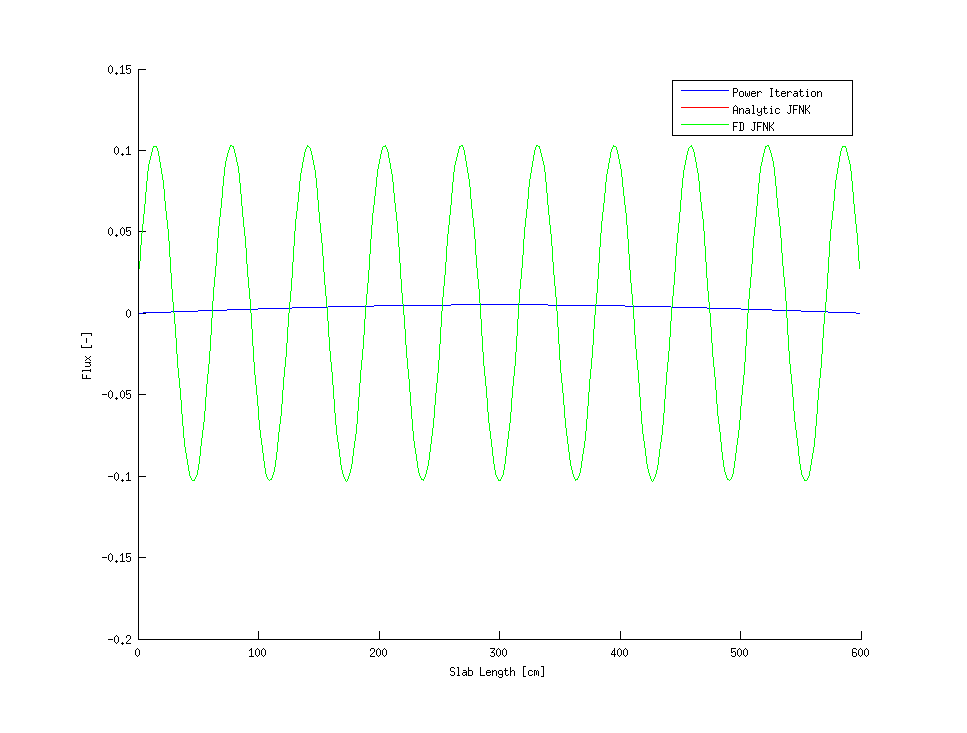
\includegraphics[scale=0.5]{pics/FundMode_600}
\par\end{centering}

\caption{Flux Eigenvector Comparison, 600 cm}


\label{fig:fluxmode}
\end{figure}
 The results show that Newton-based methods do not agree with the
power iteration even though the residual criteria is met. This is
because any eigenvalue/eigenvector pair satisfies the residual equations.
To verify, the $\mathtt{eigs}$ command in MATLAB was used to get
an array of eigenvalues of the system. Sure enough, the converged
eigenvalue was listed. To ensure that the Newton-based methods converge
to the fundamental mode, two power iterations were computed to get
the flux shape in the correct direction. After applying this, the
results look better and are shown in Figs. \ref{fig:flux600} and
\ref{fig:fluxdiff600}.
\begin{figure}
\begin{centering}
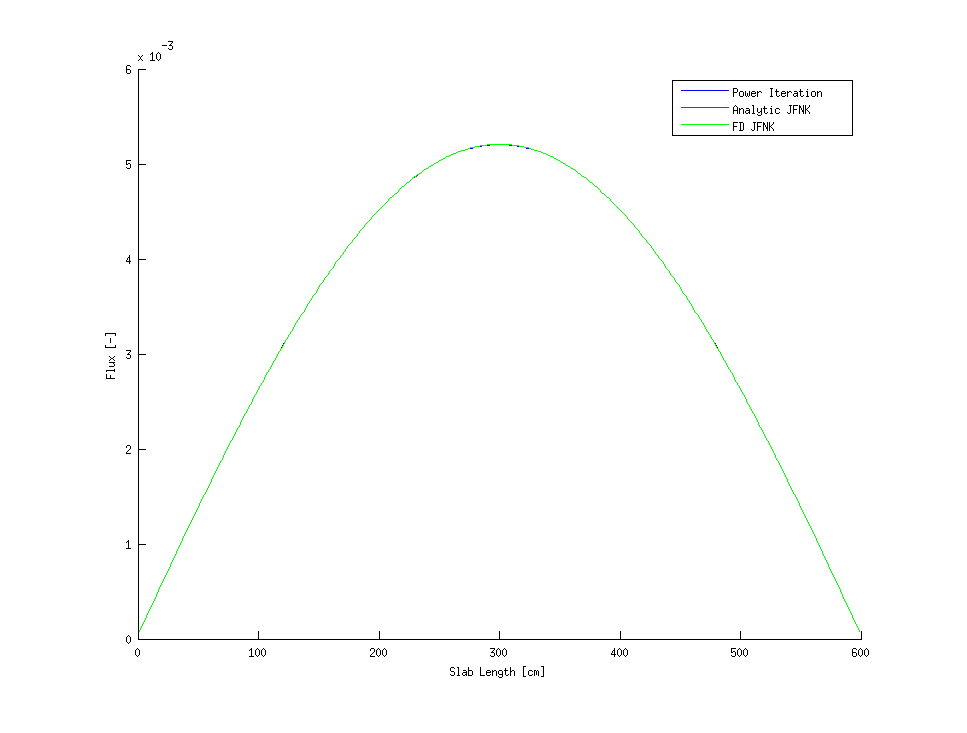
\includegraphics[scale=0.5]{pics/Flux_600}
\par\end{centering}

\caption{Comparison of Flux with Initial Power Iteration, 600 cm}


\label{fig:flux600}
\end{figure}
 
\begin{figure}
\begin{centering}
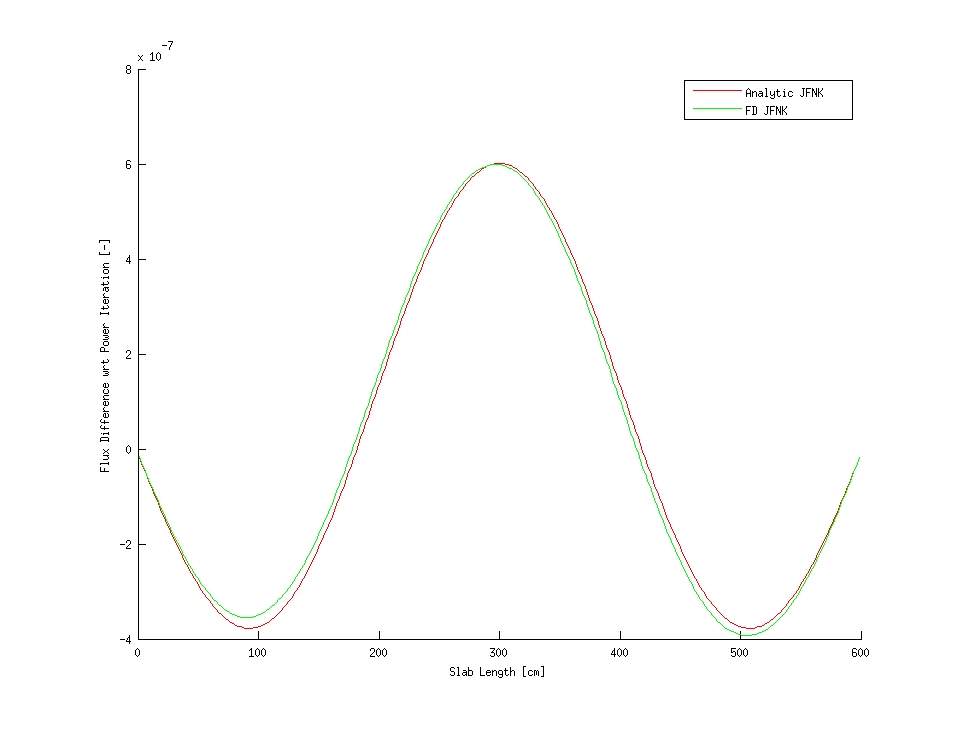
\includegraphics[scale=0.5]{pics/diff_flux_600}
\par\end{centering}

\caption{Difference of Flux with Initial Power Iteration, 600 cm}


\label{fig:fluxdiff600}
\end{figure}
 The differences in the plot with respect to power iteration are within
the converged nonlinear iteration tolerance of $10^{-6}$. What is
more interesting to compare is number of iterations, final residual
and computational time. These results are listed in Table \ref{tab:eigcomp_600}.
\begin{table}
\caption{Comparison of Methods to Solve Neutronic Eigenvalue Problem, 600 cm}


\begin{centering}
\begin{tabular}{cccc}
\toprule 
Method & Iterations & Final Residual & Time {[}s{]}\tabularnewline
\midrule
\midrule 
Power Iteration & 984 & $9.9997\times10^{-7}$ & 0.116\tabularnewline
\midrule 
Analytic JFNK & 6 & $5.024\times10^{-7}$ & 0.075\tabularnewline
\midrule 
Finite Difference JFNK & 6 & $4.2829\times10^{-7}$ & 0.147\tabularnewline
\bottomrule
\end{tabular}
\par\end{centering}

\label{tab:eigcomp_600}
\end{table}
 From the results, the power iteration takes almost 1000 iterations.
This is because the rate of convergence of power iteration is inversely
proportional to the dominance ratio. The closer the dominance ratio
is to unity, the more iterations it will take to converge. The analytic
Jacobian-free method performs the best with respect to computational
time. The finite difference version of JFNK does not do as well as
the analytic multiplication. However, the time it takes to do this
is very comparable to power iteration. Both method (2) and method
(3) will be compared again in the coupled neutrons/thermal hydraulics
problem.

The slab width was then decreased to 370 cm which is about the length
of the active fuel rod length producing power in a standard pressurized
water reactor. The dominance ratio of this system is 0.992. The difference
in the the flux eigenvectors is shown in Fig. \ref{fig:fluxcmp_300}.
\begin{figure}
\begin{centering}
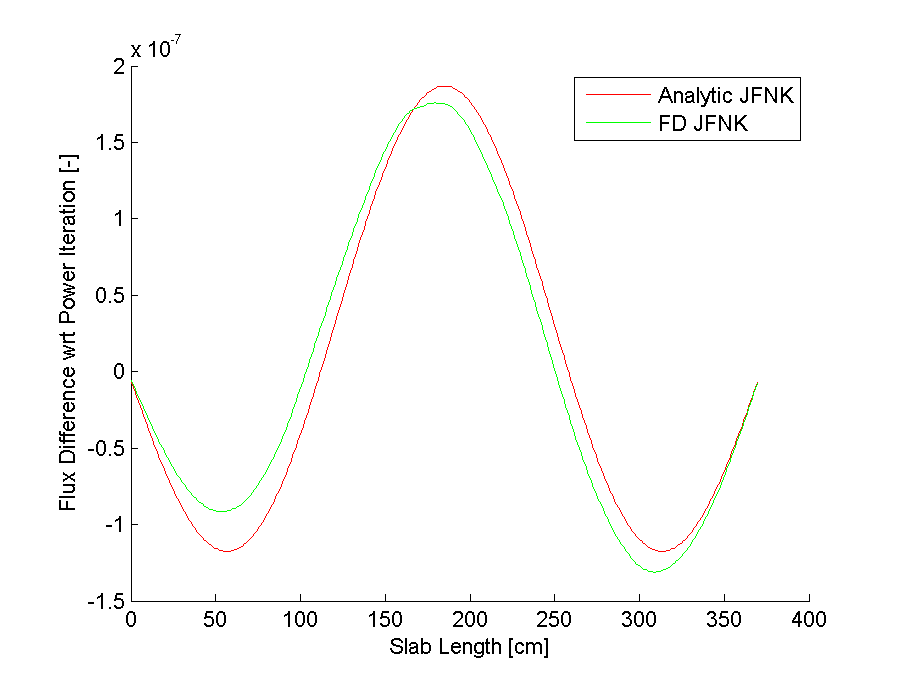
\includegraphics[scale=0.5]{pics/diff_flux_300}
\par\end{centering}

\caption{Flux Eigenvector Comparison, 300 cm}


\label{fig:fluxcmp_300}
\end{figure}
 A comparison of the number of iterations, final residual and computation
time is presented in Table \ref{tab:eigcomp_300}.
\begin{table}
\caption{Comparison of Methods to Solve Neutronic Eigenvalue Problem, 300 cm}


\begin{centering}
\begin{tabular}{cccc}
\toprule 
Method & Iterations & Final Residual & Time {[}s{]}\tabularnewline
\midrule
\midrule 
Power Iteration & 424 & $9.9881\times10^{-7}$ & 0.07037\tabularnewline
\midrule 
Analytic JFNK & 5 & $5.024\times10^{-7}$ & 0.05714\tabularnewline
\midrule 
Finite Difference JFNK & 5 & $4.2829\times10^{-7}$ & 0.08562\tabularnewline
\bottomrule
\end{tabular}
\par\end{centering}

\label{tab:eigcomp_300}
\end{table}
 From the results, the time to perform the power iteration method
takes fewer iterations than in the high dominance ratio case. Therefore,
it is observed that the dominance ratio of the system has a direct
effect on how long the power iteration takes. Both JFNK methods took
the same amount of iterations, with the finite difference approach
taking slightly longer to solve. This is due to the number of GMRES
inner iterations needed to converge the system. The JFNK method was
therefore successfully applied to the neutronics eigenvalue problem.


\section{Steady-State Coupled Physics Solution}

In this section the determination of the steady-state spatial distribution
of flux, power temperature and density will be determined. Equations
(\ref{eq:NeutronOper}), (\ref{eq:norm}), (\ref{eq:normfluxdiscrete}),
(\ref{eq:energyoper}), (\ref{eq:TempOper}), (\ref{eq:DensityTempVec}),
(\ref{eq:AbsRHOCellVec}), (\ref{eq:NfissRHOCellVec}), (\ref{eq:DiffRHOCellVec})
and (\ref{eq:KfissRHOCellVec}) comprise the set of equations needed
to solve for the steady distributions. The residual equations can
then be formulated as

\begin{equation}
\mathbf{F}=\left[\begin{array}{c}
\mathbb{M}\mathbf{\Phi}-\lambda\mathbb{F}\mathbf{\Phi}\\
Q_{R}-\tilde{c}\kappa\mathbf{\Sigma}_{f}^{\mathrm{T}}\mathbf{\Phi}\Delta x.\\
\mathbf{Q}-\tilde{c}\mathbb{E}\mathbf{\Phi}\Delta x\\
\mathbb{S}\mathbf{T}-\mathbb{R}\mathbf{Q}\\
\mathcal{P}-\rho\left(\mathbf{T},p\right)\\
\mathbf{\Sigma}_{a}-\Sigma_{a}^{ref}-\frac{\partial\Sigma_{a}}{\partial\rho}\left[\mathcal{P}-\rho^{ref}\right]\\
\nu\mathbf{\Sigma}_{f}-\nu\Sigma_{f}^{ref}-\frac{\partial\nu\Sigma_{f}}{\partial\rho}\left[\mathcal{P}-\rho^{ref}\right]\\
\mathbf{D}-D^{ref}-\frac{\partial D}{\partial\rho}\left[\mathcal{P}-\rho^{ref}\right],\\
\kappa\mathbf{\Sigma}_{f}-\kappa\Sigma_{f}^{ref}-\frac{\partial\kappa\Sigma_{f}}{\partial\rho}\left[\mathcal{P}-\rho^{ref}\right]\\
-\frac{1}{2}\mathbf{\Phi}^{\mathrm{T}}\mathbf{\Phi}+\frac{1}{2}
\end{array}\right].\label{eq:residualStatic}
\end{equation}
Note that in the nonlinear equations, the operators $\mathbb{M}$,
$\mathbb{F}$ and $\mathbb{E}$ have to updated since they depend
on neutronic parameters. These residual equations are written in a
function in MATLAB and can be called during the Newton iteration.
The unknown vector is then constructed as

\begin{equation}
\mathbf{x}=\left[\begin{array}{c}
\mathbf{\Phi}\\
\tilde{c}\\
\mathbf{Q}\\
\mathbf{T}\\
\mathcal{P}\\
\mathbf{\Sigma}_{a}\\
\nu\mathbf{\Sigma}_{f}\\
\mathbf{D}\\
\kappa\mathbf{\Sigma}_{f}\\
\lambda
\end{array}\right].\label{eq:unknownStatic}
\end{equation}
 From the residual vector and unknown vector, the analytic Jacobian-vector
product can be constructed in matrix notation as

{\small 
\begin{equation}
\mathbb{J}\mathbf{y}=\left[\begin{array}{c|c|c|c|c|c|c|c|c|c}
\mathbb{M}-\lambda\mathbb{F} & 0 & 0 & 0 & 0 & \mathrm{diag\left\{ \mathbf{\Phi}\right\} } & -\lambda\mathrm{diag\left\{ \mathbf{\Phi}\right\} } & \mathbb{MD} & 0 & -\mathbb{F}\mathbf{\Phi}\\
\hline -\tilde{c}\kappa\mathbf{\Sigma}_{f}^{\mathrm{T}}\Delta x & -\kappa\mathbf{\Sigma}_{f}^{\mathrm{T}}\mathbf{\Phi}\Delta x & 0 & 0 & 0 & 0 & 0 & 0 & -\tilde{c}\mathbf{\Phi}^{\mathrm{T}}\Delta x & 0\\
\hline -\mathbb{E}\tilde{c}\Delta x & -\mathbb{E}\mathbf{\Phi}\Delta x & \mathbb{I} & 0 & 0 & 0 & 0 & 0 & -\tilde{c}\Delta x\mathrm{diag}\left\{ \mathbf{\Phi}\right\}  & 0\\
\hline 0 & 0 & -\mathbb{R} & \mathbb{S} & 0 & 0 & 0 & 0 & 0 & 0\\
\hline 0 & 0 & 0 & -\rho\left(T\right)* & \mathbb{I} & 0 & 0 & 0 & 0 & 0\\
\hline 0 & 0 & 0 & 0 & -\frac{\partial\Sigma_{a}}{\partial\rho}\mathbb{I} & \mathbb{I} & 0 & 0 & 0 & 0\\
\hline 0 & 0 & 0 & 0 & -\frac{\partial\nu\Sigma_{f}}{\partial\rho}\mathbb{I} & 0 & \mathbb{I} & 0 & 0 & 0\\
\hline 0 & 0 & 0 & 0 & -\frac{\partial D}{\partial\rho}\mathbb{I} & 0 & 0 & \mathbb{I} & 0 & 0\\
\hline 0 & 0 & 0 & 0 & -\frac{\partial\Sigma_{a}}{\partial\rho}\mathbb{I} & 0 & 0 & 0 & \mathbb{I} & 0\\
\hline -\mathbf{\Phi}^{\mathrm{T}} & 0 & 0 & 0 & 0 & 0 & 0 & 0 & 0 & 0
\end{array}\right]\left[\begin{array}{c}
y_{\phi}\\
y_{\tilde{c}}\\
y_{Q}\\
y_{T}\\
y_{\rho}\\
y_{\Sigma_{a}}\\
y_{\nu\Sigma_{f}}\\
y_{D}\\
y_{\kappa\Sigma_{f}}\\
y_{\lambda}
\end{array}\right]\label{eq:JacobianStatic}
\end{equation}
 }Performing the Jacobian-vector product analytically, the set of
equations is

\begin{equation}
\mathbb{J}\mathbf{y}=\left[\begin{array}{c}
\left(\mathbb{M}-\lambda\mathbb{F}\right)y_{\phi}+\left(\mathrm{diag\left\{ \mathbf{\Phi}\right\} }\right)y_{\Sigma_{a}}+\left(-\lambda\mathrm{diag\left\{ \mathbf{\Phi}\right\} }\right)y_{\nu\Sigma_{f}}+\left(\mathbb{MD}\right)y_{D}+\left(-\mathbb{F}\mathbf{\Phi}\right)y_{\lambda}\\
\left(-\tilde{c}\kappa\mathbf{\Sigma}_{f}^{\mathrm{T}}\Delta x\right)y_{\phi}+\left(-\kappa\mathbf{\Sigma}_{f}^{\mathrm{T}}\mathbf{\Phi}\Delta x\right)y_{\tilde{c}}+\left(-\tilde{c}\mathbf{\Phi}^{\mathrm{T}}\Delta x\right)y_{\kappa\Sigma_{f}}\\
\left(-\mathbb{E}\tilde{c}\Delta x\right)y_{\phi}+\left(-\mathbb{E}\mathbf{\Phi}\Delta x\right)y_{\tilde{c}}+\left(\mathbb{I}\right)y_{Q}+\left(-\tilde{c}\Delta x\mathrm{diag}\left\{ \mathbf{\Phi}\right\} \right)y_{\kappa\Sigma_{f}}\\
\left(-\mathbb{R}\right)y_{Q}+\left(\mathbb{S}\right)y_{T}\\
\left[-\rho\left(T\right)*\right]y_{T}+\left(\mathbb{I}\right)y_{\rho}\\
\left(-\frac{\partial\Sigma_{a}}{\partial\rho}\mathbb{I}\right)y_{\rho}+\left(\mathbb{I}\right)y_{\Sigma_{a}}\\
\left(-\frac{\partial\nu\Sigma_{f}}{\partial\rho}\mathbb{I}\right)y_{\rho}+\left(\mathbb{I}\right)y_{\nu\Sigma_{f}}\\
\left(-\frac{\partial D}{\partial\rho}\mathbb{I}\right)y_{\rho}+\left(\mathbb{I}\right)y_{D}\\
\left(-\frac{\partial\kappa\Sigma_{f}}{\partial\rho}\mathbb{I}\right)y_{\rho}+\left(\mathbb{I}\right)y_{\kappa\Sigma_{f}}\\
\left(-\mathbf{\Phi}^{\mathrm{T}}\right)y_{\phi}
\end{array}\right]\label{eq:JacobianVectStatic}
\end{equation}
 This Jacobian-vector operation is performed in a MATLAB function
that can be called upon by the GMRES solver. In Eqs. (\ref{eq:JacobianStatic})
and (\ref{eq:JacobianVectStatic}):
\begin{itemize}
\item $\mathrm{diag}\{\}$ is the diagonal operator that places a vector
along the diagonal of a matrix,
\item $\mathbb{MD}$ is the partial derivative of the operator $\mathbb{M}$
with respect to the diffusion coefficient,
\item $\mathbb{I}$ is the identity matrix,
\item $\left[-\rho\left(T\right)*\right]y_{T}$ is the partial derivative
of the state equation with respect to temperature and must be handled
with a finite difference.
\end{itemize}
The $\mathbb{MD}$ operator has the following form for the boundaries
and interior cells:
\begin{itemize}
\item Left boundary
\begin{equation}
\left(\frac{2}{\Delta x^{2}}\frac{D_{2}^{2}}{\left(D_{2}+D_{1}\right)^{2}}+2\frac{\left(1-\beta\right)^{2}}{\left[4D_{1}\left(1+\beta\right)+\Delta x\left(1-\beta\right)\right]^{2}}\right)\bar{\phi}_{1}-\frac{2}{\Delta x^{2}}\frac{D_{2}^{2}}{\left(D_{2}+D_{1}\right)^{2}}\bar{\phi}_{2},
\end{equation}
 
\item Interior
\begin{equation}
-\frac{2}{\Delta x^{2}}\frac{D_{i-1}^{2}}{\left(D_{i}+D_{i-1}\right)^{2}}\bar{\phi}_{i-1}+\left(\frac{2}{\Delta x^{2}}\frac{D_{i+1}^{2}}{\left(D_{i+1}+D_{i}\right)^{2}}+\frac{2}{\Delta x^{2}}\frac{D_{i-1}^{2}}{\left(D_{i}+D_{i-1}\right)^{2}}\right)\bar{\phi}_{i}-\frac{2}{\Delta x^{2}}\frac{D_{i+1}^{2}}{\left(D_{i+1}+D_{i}\right)^{2}}\bar{\phi}_{i+1},
\end{equation}

\item Right boundary
\begin{equation}
-\frac{2}{\Delta x^{2}}\frac{D_{I-1}^{2}}{\left(D_{I}+D_{I-1}\right)^{2}}\bar{\phi}_{I-1}+\left(2\frac{\left(1-\beta\right)^{2}}{\left[4D_{I}\left(1+\beta\right)+\Delta x\left(1-\beta\right)\right]^{2}}+\frac{2}{\Delta x^{2}}\frac{D_{I-1}^{2}}{\left(D_{I}+D_{I-1}\right)^{2}}\right)\bar{\phi}_{I}.
\end{equation}
 
\end{itemize}
Each of these equations will be placed on the diagonal of the $\mathbb{MD}$
matrix. The last tricky part is that the partial derivative of the
state equation is not known. Therefore, this section will have to
be evaluated with a finite difference and has the form,

\begin{equation}
\left[-\rho\left(T\right)*\right]y_{T}=\frac{\left[\mathcal{P}-\rho\left(\mathbf{T}+\epsilon y_{T},p\right)\right]-\left[\mathcal{P}-\rho\left(\mathbf{T},p\right)\right]}{\epsilon}.
\end{equation}
 The overall algorithm to solve this problem is presented in Algorithm
\ref{alg:steadycoupled}. 
\begin{algorithm}
\caption{Steady State Coupled Solution }


\begin{algorithmic}[1]
\STATE read input
\STATE perform small number of power iterations to estimate flux shape
\STATE compute thermal hydraluics based off flux shape
\STATE form approximate Jacobian and perform ILU to get preconditioner
\STATE perform Newton Iterations
\end{algorithmic}

\label{alg:steadycoupled}
\end{algorithm}
 Once the user-defined input file is set, the code runs a few power
iterations to get the gross shape of the flux correct without feedback
for an initial guess to the Newton solver. An initial guess of the
thermal hydraulics is also computed based on this guessed flux shape.
In order to minimize the number of inner iterations in the GMRES solver,
a preconditioner must be determined. Since the Jacobian is never formed
in the Newton iteration loop, this preconditioner cannot be computed
on-the-fly. Also, it would be expensive to recompute a preconditioner
at every Newton step. Therefore, the preconditioner is only formed
once using the initial guess values. Here, the approximate Jacobian
is fully constructed and ILU factorization is performed. This constant
preconditioner is then used in the GMRES solver at every Newton iteration. 

The solution of this steady state problem took about 7.06 seconds
to complete, with 8 total Newton iterations and about 21 inner GMRES
iterations on average. The results of this calculation are presented
in Figs. \ref{fig:coupledSteady1} and \ref{fig:coupledSteady2}.
\begin{figure}
\begin{centering}
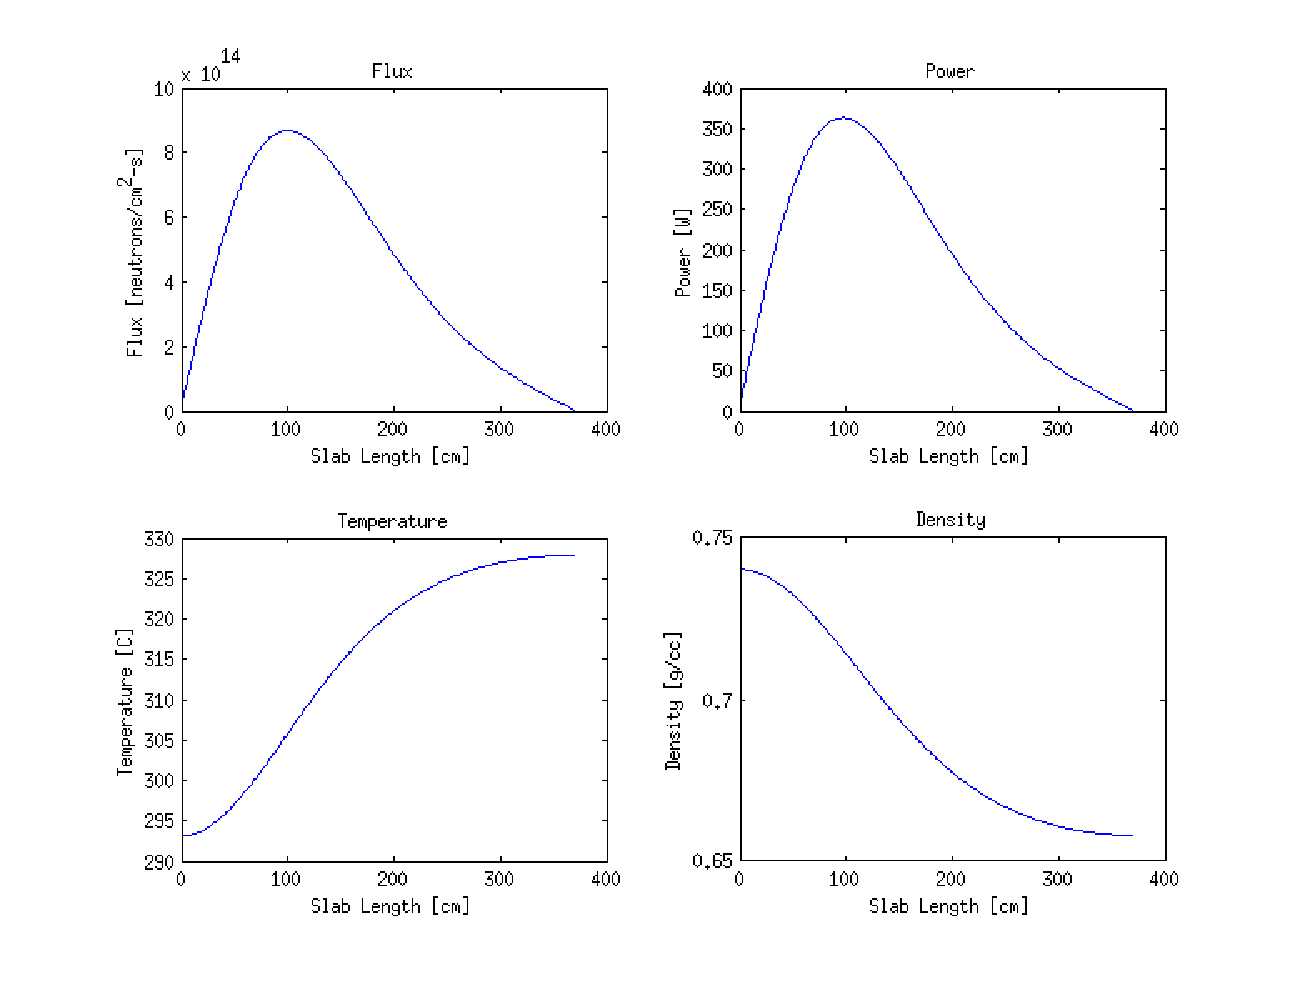
\includegraphics[scale=0.5]{pics/SteadyCoupledb}
\par\end{centering}

\caption{Results from Steady State Calculation Part 1}


\label{fig:coupledSteady1}
\end{figure}
 
\begin{figure}
\begin{centering}
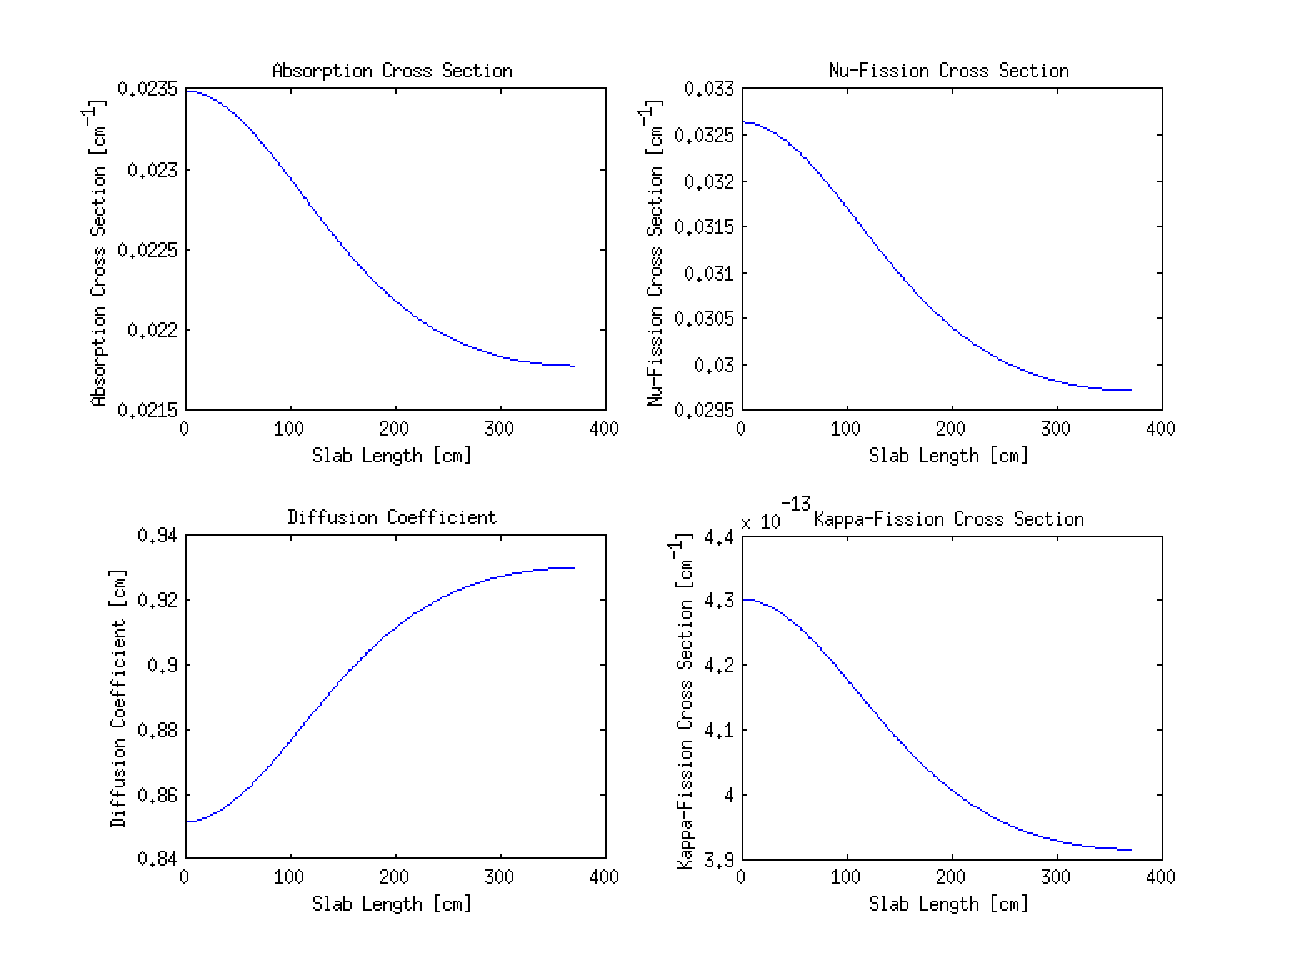
\includegraphics[scale=0.5]{pics/SteadyCoupleda}
\par\end{centering}

\caption{Results from Steady State Calculation Part 2}


\label{fig:coupledSteady2}
\end{figure}
 The results prove that the feedback is working correctly. Instead
of getting a cosine shape as with the case of no feedback (see Section
\ref{sec:steadyneut}), the cosine shape is now skewed to the left.
This is due to the density feedback, where the density of water is
higher in the left part of the slab than in the right. Therefore,
more fissions will occur to the left and more power is produced. 

The solution of this problem was not easy. If the above equations
are implemented as is, the MATLAB code will not converge on a solution.
This is primarily due to the fact that the kappa-fission cross section
is so small. It is on the order of $10^{-13}$ which is much smaller
than other quantities in the problem. Therefore, the normalization
constant is very large to scale the flux eigenvector. This makes the
problem very ill-conditioned even though a preconditioner is used.
Since the normalization constant is always multiplied by the kappa-fission
cross section in the residual equations, another constant of $10^{12}$
is applied in the input file. Therefore, the span of the magnitudes
of the flux-to-power normalization constant and kappa-fission cross
section will be smaller. This proved to be effective for this situation
and was used to compute the results presented in this section. 

Finally, it is interesting to look at the distribution of how time
was spent in the code. To do this, MATLAB's built in profiler was
used. The results of the profiler are shown in Fig. \ref{fig:profileSteady}.
\begin{figure}
\begin{centering}
\includegraphics[scale=0.2]{pics/Profile_Steady}
\par\end{centering}

\caption{Profiler Results for Steady-State Case}


\label{fig:profileSteady}
\end{figure}
 From the results, it is interesting to see that approximately 88\%
of the time was spent in the lookup XSteam tables to relate density
to temperature. Unfortunately, nothing can be done about this if the
lookup tables are going to be used. An improvement on this would be
to fit the density vs. temperature data with a polynomial in the range
of interest and use that in the residual equations and Jacobian-vector
product routines.


\section{Transient Coupled Physics Solution}


\section{Conclusions}

\bibliographystyle{plain}
\bibliography{refs}

\end{document}
